%%%%%%%%%%%%%%%%%%%%%%%%%%%%%%%%%%%%%%%%%%%%%%%%%%%%%%%%%%%%%%%%%
%%% %
%%% % weiiszablon.tex
%%% % The Faculty of Electrical and Computer Engineering
%%% % Rzeszow University Of Technology diploma thesis Template
%%% % Szablon pracy dyplomowej Wydziału Elektrotechniki 
%%% % i Informatyki PRz
%%% % June, 2015
%%%%%%%%%%%%%%%%%%%%%%%%%%%%%%%%%%%%%%%%%%%%%%%%%%%%%%%%%%%%%%%%%

\documentclass[12pt,twoside]{article}
\usepackage{cite}
\usepackage{weiiszablon}

\author{Bartłomiej Mateusz Paluch}

% np. EF-123456, EN-654321, ...
\studentID{EF-160786}

\title{Zastosowanie architektury mikroserwisowej oraz konteneryzacji w tworzeniu i wdrażaniu aplikacji webowej}
\titleEN{The use of microservice architecture and containerization in the implementation and deployment of a web application}


%%% wybierz rodzaj pracy wpisując jeden z poniższych numerów: ...
% 1 = inżynierska	% BSc
% 2 = magisterska	% MSc
% 3 = doktorska		% PhD
%%% na miejsce zera w linijce poniżej
\newcommand{\rodzajPracyNo}{1}


%%% promotor
\supervisor{dr inż. Tomasz Krzeszowski prof. PRz}
%% przykład: dr hab. inż. Józef Nowak, prof. PRz

%%% promotor ze stopniami naukowymi po angielsku
\supervisorEN{Tomasz Krzeszowski, PhD, Eng., Associate Prof.}

\abstract{Praca miała na celu sprawdzenie możliwości zastosowań wzorca architektury mikroserwisowej oraz konteneryzacji w tworzeniu i wdrażaniu aplikacji webowych. W ramach pracy utworzono prototyp aplikacji w postaci stosu skonteneryzowanych mikroserwisów wdrożonego w chmurowym klastrze publicznym pozwalający na sprawdzenie zastosowań konteneryzacji i mikroserwisów. W ramach wdrożenia utworzono pliki na klaster \texttt{kubernetes} i wykonano wdrożenie stosu w klastrze lokalnym i publicznym. Następnie opisano zastosowania wynikające z testów. Na koniec wyszczególniono zalecenia autora dotyczące zastosowań sprawdzanych zagadnień. }
\abstractEN{The aim of the work was to check the applicability of the microservice architecture pattern and containerization in the creation and implementation of web applications. As part of the work an application prototype was created in the form of a stack of containerized microservices implemented in a public cloud cluster that allows the study of applications of containerization and microservices. As part of the deployment examining, the files for kubernetes cluster were created and the deployment of the microservice stack was performed on a local and public cluster. Then, the applications resulting from the research are described. Finally, the author's recommendations for applications of the checked issues are listed.}

\begin{document}

% strona tytułowa
\maketitle

\blankpage

% spis treści
\tableofcontents

\clearpage
\blankpage


\section*{Wykaz symboli, oznaczeń i skrótów}
\addcontentsline{toc}{section}{Wykaz symboli, oznaczeń i skrótów}%
Mapowanie obiektowo relacyjne (ang. \textit{Object Relational Model}, \textit{ORM}) jest narzędziem konwersji modeli na odpowiadające im pola typów danych w bazie danych. Wiele narzędzi \texttt{ORM} pozwala na utworzenie modelu tworzącego automatycznie odpowiedni schemat w bazie danych.

\textit{AKS} (ang. \textit{Azure Kubernetes Service}) — chmurowa implementacja klastra \texttt{kubernetes} w ramach platformy \texttt{Azure} od \texttt{Microsoftu}.

Model — jest to obiekt o określonym schemacie, odpowiadający zawartości schematu tabeli w bazie danych.

Widok — wykorzystywany w kontekście frameworku w \texttt{Django}, odpowiada za logikę biznesową aplikacji.

Byt (ang. \textit{Entity}) — nazwa własna w \texttt{Javie} dla modelu \texttt{ORM}. 

Repozytorium — w kontekście Springa jest interfejsem obsługi bazy danych dla określonych bytów.

\textit{API} (ang. \textit{Application Programming Interface}) — interfejs programowania aplikacji, w kontekście pracy wykorzystywane jest \texttt{API REST}.

\textit{REST} (ang. \textit{Representational State Transfer}) — styl pisania aplikacji bezstanowych w oparciu o reguły dotyczące sposobu użycia metod protokółu \texttt{HTTP}.

Broker wiadomości (ang. \textit{message broker}) — ,,pośrednik wiadomości'', ze względu na popularność nazwy w środowisku programistycznym i literaturze wykorzystywana jest ta nazwa. Służy do przesyłania wiadomości pomiędzy aplikacjami w sposób asynchroniczny — bez konieczności oczekiwania na odpowiedź.

Kafka — broker wiadomości wykorzystywany w pracy.

Temat — jest to implementacja miejsca w instancji aplikacji brokera \texttt{Apache Kafka} przechowująceego wiadomości.

Konsument — jest to klient aplikacji odczytujący informacje z tematu kafki.

Producent — jest to klient aplikacji wysyłający informację na temat kafki.

\textit{KIND} (ang. \textit{kubernetes in the docker}) — \texttt{kubernetes} w \texttt{dokerze}, skrót nazwy dla implementacji klastra \texttt{kubernetes} wewnątrz \texttt{dockera}.

Serwis — w kontekście aplikacji spring jest to komponent implementujący funkcjonalność biznesową, w kontekście \texttt{kubernetes} jest to usługa udostępniająca sieć wdrożeniom, w kontekście mikroserwisów implementacja pojedynczego mikroserwisu.

\textit{Domain-Driven Design} — podejście do projektowania aplikacji na bazie domen biznesowych — obiektów w aplikacji utworzonych na podstawie zachowań obiektów istniejących w rzeczywistości.

Wydarzenie domenowe — funkcjonalność systemu opisana jako wydarzenie, dla przykładu może to być dodanie produktu do koszyka, zalogowanie użytkownika.

\textit{Event Storming} — technika pozwalająca na określenie domen biznesowych przy pomocy grupowania wydarzeń domenowych mających miejsce w systemie w obiekty domenowe wspierające ich obsługę.

Demon - jest to proces unixowy, nie wymagający interakcji użytkownika do jego działania.

\textit{CLI docker} (ang. \text{Command Line Interface}) — interfejs demona linii poleceń \texttt{docker}.

\clearpage

\section{Wstęp}

Aktualnie dostrzegalny postęp i rozwój technologiczny, powstały poprzez rozwój przemysłu 4.0 oraz Internetu rzeczy, stawia wysokie wymagania względem twórców oprogramowania komputerowego.
Wytwarzane oprogramowanie ma być produkowane szybko, jednolicie oraz pozwalać na niemal natychmiastowe wdrożenie nowej wersji tworu na serwer produkcyjny. Tworzone aplikacje powinny być jak najbardziej niezależne od siebie, a rozwój ich nowych modułów nie powinien wiązać się z koniecznością zmiany tysięcy linijek kodu w uprzednio powstałych elementach aplikacji. Dodatkowo środowisko deweloperskie oraz sposób wdrożenia nie może pozwalać na sytuację gdzie to samo oprogramowanie nie działa ze względu na urządzenie, sterowniki, system operacyjny lub konfigurację.

Powstawanie błędów w trakcie pracy, których geneza jest trudna w odnalezieniu lub uciążliwa w znalezieniu, doprowadza do zmarnowania wielu cennych godzin rozwoju na walkę z problemami, które nie dają żadnych wartości biznesowych, co efektownie przedłuża czas tworzenia aplikacji. Co więcej, im dłużej rozwijamy oprogramowanie, tym więcej technologii zostaje wprowadzonych, a co za tym idzie programiści spędzają dłuższy czas nad konfiguracją i wprowadzeniem zmian w środowisku deweloperskim.

Sposób tworzenia oprogramowania w architekturze monolitycznej, polegający na utworzeniu jednego spójnego systemu wymaga dużej wiedzy o strukturze i sposobie działania wszystkich elementów wielkiej aplikacji. Niejednokrotnie okazuje się, że niewielka zmiana potrafi okazać się niemożliwa w implementacji lub całkowicie nieopłacalna. Co więcej, wyszkolenie nowego pracownika i przygotowanie go do pracy nad tak tworzonym systemem, który wymaga znajomości wszystkich zastosowanych algorytmów i ograniczeń narzuconych przez elementy systemu rozwinięte przez cały cykl czasu życia aplikacji jest czasochłonne i bardzo kosztowne. Utrata takiego pracownika może wiązać się z niebezpieczeństwem całkowitej porażki założeń projektowych.

Zastosowanie monolitycznego podejścia powoduje w pewnej fazie rozwoju oprogramowania niemożliwość zmiany stosu technologicznego lub przeogromne koszty z tym związane. Dodatkowo brak funkcjonalności lub awaria jednego elementu aplikacji powoduje, że cały system przestaje działać.

Celem przeciwdziałaniu tym problemom powstał wzorzec architektury mikroserwisowej. Architektura ta zakłada tworzenie aplikacji w zasięgu domeny biznesowej lub obsługi pojedynczej funkcji biznesowej z zastosowaniem luźnych powiązań pomiędzy mikroserwisami.

Wprowadzenie mikroserwisowego podejścia do tworzenia aplikacji jest nowoczesnym sposobem mającym w zamyśle poradzić sobie z większością wyżej wymienionych problemów tworzenia aplikacji. Podejście to pozwala na separację stosu technologicznego i funkcjonalności do mikroserwisów — pojedynczych modułów aplikacji zorientowanych na zdolność biznesową, które są wdrażane oddzielnie przez zautomatyzowaną maszynerię\cite{fowler,fowler2}.

Utworzenie wielu mikroserwisów wiąże się z uzyskaniem wielu środowisk operacyjnych. Rozwiązaniem tego problemu jest użycie konteneryzacji w procesie rozwoju i wdrożenia aplikacji. Konteneryzacja polega na utworzeniu niezależnego wirtualnego środowiska systemowego\cite{virtualisation}. Różni się ona od popularnie wykorzystywanej wirtualizacji tym, że kontenery współdzielą system i zasoby systemowe, na którym są uruchomione. Kontener nie jest pełnym systemem operacyjnym tak jak maszyna wirtualna, wykorzystuje on tylko niezbędne elementy takie jak biblioteki wykorzystywane w pozostałych aplikacjach przez co, zużywa mniejsze zasoby oraz pozwala na jednoczesne uruchomienie większej liczby środowisk jednocześnie\cite{differences}.

Użycie konteneryzacji przy tworzeniu aplikacji w architekturze mikroserwisowej jest kluczowym elementem uzyskania separacji środowiskowej pomiędzy mikroserwisami w środowisku lokalnym. Brak utworzenia separacji środowiskowej pomiędzy mikroserwisami. Powoduje to tak naprawdę utworzenie rozproszonego monolitu, który jest trudny w utrzymaniu ze względu na brak określonych informacji o zależnościach systemowych znajdujących się w innych mikroserwisach. Efektem tego mogą być niespodziewane efekty uboczne.

Niestety, tak jak każde rozwiązanie i to powoduje własne problemy. Wdrożenie skonteneryzowanych mikroserwisów na wielu serwerach, w celu uzyskania redundancji jest niesamowicie trudne. Do pewnego momentu przy wielkich systemach był to problem prawie nierozwiązywalny. Konieczność konfiguracji wielu serwerów pod względem połączeń pomiędzy nimi, wymiany informacji oraz konfiguracji sposobu w jaki ustalić, która usługa ma mieć dostęp do innej, była rzeczą niesamowicie czasochłonną. Do rozwiązania tego problemu zaprojektowano klastry \texttt{kubernetes}. Klastrem \texttt{kubernetes} nazywamy grupę węzłów serwerowych działających jako jeden system do uruchamiania skonteneryzowanych aplikacji\cite{cluster}.

Wewnątrz klastra nie ma podziału na poszczególne serwery. Wszystkie urządzenia spięte w ramach klastra widoczne są jako jeden serwer z identyczną konfiguracją. Zasoby serwerów są współdzielone i widoczne jako jednolita całość. 

Informacje udostępniane o klastrach \texttt{kubernetes} są zazwyczaj skoncentrowane na sposobie ich użycia. Dzieje się tak, ponieważ utworzenie własnego klastra wymaga odpowiedniej infrastruktury, zespołu specjalistów do tworzenia i utrzymania klastra. Istnienie tanich rozwiązań chmurowych implementujących fizyczny klaster powoduje, że utworzenie własnego klastra jest prawie nieopłacalne. Dodatkowo usługodawcy nie dzielą się wiedzą jak utworzyć klaster z użyciem własnej infrastruktury, byłoby to dla nich utratą potencjalnego klienta. Z tego powodu w pracy wykorzystano usługi jednego z wiodących dostawców, \texttt{Azure Kubernetes Service}.

 W związku z tym, że tworzenie aplikacji rozproszonych jest głównie wykorzystywane przez programistów z wieloletnim doświadczeniem, większość przykładów dotyczących implementacji dotyczy określonych sytuacji biznesowych. Powstałe w ten sposób przykłady nie nadają się do analizy tematu przez niedoświadczonego programistę. Dodatkowym powodem wyboru tego tematu jest fakt spędzenia wielu godzin przy pracy nad tworzeniem aplikacji z wykorzystaniem architektury mikroserwisowej.

Praca ma edukacyjny charakter praktyczny. Powstała w celu zapoznania się z tematem oraz udostępnienia tych informacji szerszej publiczności.

Praca składa się z czterech rozdziałów:
\begin{enumerate}[label=\arabic*), leftmargin=1.25cm]
\item wstęp — opisuje rozdziały i podrozdziały, problematykę tematu oraz określa zakres i cel pracy;
\item mikroserwisy i konteneryzacja — teoretyczna część pracy, wprowadza w zagadnienia związane z pracą. Zawiera aktualny stan wiedzy oraz wiedzę dotyczącą mikroserwisów, konteneryzacji i \texttt{kubernetes}.
\item Tworzenie i wdrażanie skonteneryzowanego stosu mikroserwisów — praktyczna część pracy. Zawiera implementację stosu aplikacji wraz z opisem wdrożenia go w chmurę publiczną. Umieszczono tutaj rysunki wyników pracy oraz wykryte zastosowania przy tworzeniu i wdrażaniu aplikacji webowych.
\item podsumowanie i wnioski końcowe — zawiera informacje o tym co udało się dokonać podczas pisania pracy oraz wkład własny autora.
\end{enumerate}
\clearpage

Zakres pracy obejmował:
\begin{enumerate}[label=\arabic*), leftmargin=1.25cm]
\item utworzenie usług mikroserwisowych w różnych językach programowania,
\item nawiązanie połączeń synchronicznych i asynchronicznych pomiędzy mikrousługami przy wykorzystaniu wybranych technologii,
\item utworzenie lokalnych środowisk uruchomieniowych dla utworzonych mikroserwisów,
\item konteneryzację aplikacji,
\item przygotowanie pliku \texttt{docker-compose}, upraszczającego uruchomienie lokalnych kontenerów,
\item utworzenie konfiguracji dla mikroserwisów i wykorzystywanych usług w ramach wdrożenia lokalnego klastra \texttt{kubernetes},
\item modyfikację konfiguracji do wdrożenia w ramach wybranego rozwiązania chmurowego klastra \texttt{kubernetes} w przestrzeni publicznej,
\item utworzenie instrukcji wdrożenia oraz wdrożenie skonteneryzowanej aplikacji w klastrze chmurowym,
\item sprawdzenie możliwości i określenie zastosowań zagadnień umieszczonych w temacie.
\end{enumerate}

Praca inżynierska jest projektem mającym na celu utworzenie prototypu systemu aplikacji rozproszonej w architekturze mikroserwisowej wdrożonej z zastosowaniem konteneryzacji. Prototyp ma dodatkowo zostać wykorzystany w celu poznania wykorzystań tych rozwiązań w tworzeniu aplikacji webowych z uwzględnieniem zalet i problemów wynikających z ich zastosowania.
\clearpage
\section{Mikroserwisy i konteneryzacja}

W ramach pracy wykonano rozpoznanie dotyczące stanu wiedzy o rozwiązaniach i technologiach znajdujących się w temacie pracy. Aby przeprowadzić implementację i sprawdzić zastosowania technologii w dalszej części pracy konieczna była znajomość poniższych pojęć.

\subsection{Aktualny stan wiedzy}

Według radaru technologii, utworzonego i aktualizowanego przez \texttt{Thoughtworks}\cite{thoughtwork} — firmę konsultingową wprowadzającej nowoczesne strategie, konstrukcje oraz inżynierie oprogramowania w przedsiębiorstwach dookoła świata konteneryzacja oraz klastry \texttt{kubernetes} są rzecz wartą wprowadzenia\cite{thdocker,thkubernetes}. Architektura mikroserwisowa została przez nich określona, jako rzecz warta przetestowania w 2013 roku\cite{thservices}. Kolejne informacje można znaleść w innych wydaniach radaru pod pojęciami szczególnych wzorców architektury mikroserwisowej, dla których zalecana jest ostrożność przy ich wdrażaniu\cite{thenvy,thlayered}. Pomimo tego istnieją przedsiębiorstwa, które wykorzystują mikroserwisy. Przykładem są Netflix, Google, Amazon\cite{uses}. W internecie można znaleść artykuły wielu firm i developerów opisujące, dlaczego uważają, że mikroserwisy to przyszłość rynku rozwoju oprogramowania\cite{future,future2,future3,future4}. 


\subsection{Mikroserwisy}

Pomimo tego, że naturalnym zrozumieniem mikroserwisu jest pojedyncza implementacja jakiejś funkcjonalności w tej architekturze, pod pojęciem mikroserwisów częściej ukrywane jest znaczenie wykorzystywania architektury mikroserwisowej, czyli stylu projektowania aplikacji w postaci zbioru usług, które są\cite{Richardson}:
\begin{enumerate}[label=\arabic*), leftmargin=1.25cm]
\item łatwe w utrzymywaniu — usługi powinny być niewielkich rozmiarów, z określonym jednolitym stosem technologicznym. Zachowanie tej zasady zapewnia prostotę dalszego rozwoju;
\item luźno powiązane między sobą — implementacja funkcjonalności usługi nie powinna być oparta o to, jak inny mikroserwis działa. Zapewnia to, że programiści utrzymujący dany serwis nie są zobowiązani do znajomości sposobu implementacji innych usług w obrębie danego systemu oraz umożliwia ponowne wykorzystanie elementu w innym systemie;
\item wdrażane niezależnie — powinno być możliwe uruchomienie instancji usługi bez jednoczesnej konieczności uruchomienia dodatkowej instancji innej usługi;
\item zorientowane na funkcjonalności biznesowe — zakres działania i obsługi serwisu powinien być zawężony do określonej domeny biznesowej. Oznacza to, że jeżeli mówimy o pewnym serwisie, jesteśmy w stanie powiedzieć za co on odpowiada i jakie funkcjonalności udostępnia;
\item utrzymywane przez małe zespoły — ze względu na wzrost problemów wynikających z utrzymywania koncepcji podejścia do implementacji algorytmów oraz sposobów pisania kodu w dużych zespołach aplikacja powinna być rozwijana w zespołach składających się z małej liczby osób.\end{enumerate}

Mikroserwisy pozwalają na wykorzystanie wielu różnych stosów technologicznych, środowisk, języków programowania, a nawet systemów w obrębie jednej aplikacji. Zespół zajmujący się rozwojem serwisu płatności wykorzystujący język \texttt{Java} z frameworkiem \texttt{Quarkus} może korzystać z funkcjonalności serwisu zakupów zespołu piszącego w PHP bez zmartwień o znajomość implementacyjną obiektów lub funkcji udostępniających funkcjonalność. Jedyny element potrzebny do współpracy to wiadomość lub punkt końcowy \texttt{API}.

Ze względu na rozproszony charakter serwisów architektura mikroserwisowa zakłada wykorzystanie mechanizmów lekkiej komunikacji pomiędzy serwisami, dla przykładu protokół \texttt{API HTTP} lub przesyłanie wiadomości przy użyciu brokerów. Wysoka dostępność do bibliotek wspierających protokoły sieciowe, obsługę brokerów wiadomości oraz \texttt{API} webowego powoduje, że większość języków programowania nadaje się do tworzenia mikroserwisów. Pomimo tego faktu niewiele firm decyduje się na wprowadzenie architektury mikroserwisowej w swoją aplikację.

Jednym z głównych powodów, dla którego firmy tego nie robią, jest konieczność zmiany podejścia do sposobu tworzenia oprogramowania. Zamiast jednego zwięzłego produktu tworzymy zestaw usług powiązanych ze sobą. Wzorce projektowania sprawdzające się przy typowej aplikacji monolitycznej nie sprawdzają się tak dobrze w przypadku tworzenia aplikacji rozproszonej. Często konieczne jest wypracowanie i wprowadzenie zupełnie wcześniej nieznanych wzorców w prężnie rozwijający się i w pełni działający produkt. Prowadzi to do tego, że firmy potrzebują wprowadzić zmiany zarówno w strukturze organizacyjnej firmy jak i stosie wdrożenia aplikacji.

Nie każdy może pozwolić sobie na takie zmiany. Produkt, który już istnieje zawsze potrzebuje wsparcia technicznego, tworzenia nowych funkcjonalności oraz poprawy wcześniej istniejących błędów. Wprowadzanie tak poważnych zmian bardzo często wiąże się z utrzymaniem dwóch zespołów pracujących nad tym samym rozwiązaniem. Nie zawsze konieczne jest wprowadzenie nowej wersji aplikacji od nowa, istnieje wszakże dobrze znany wzorzec aplikacji figi dusiciela \cite{stranglerFowler}, który zakłada przekazanie pojedynczych funkcjonalności innym aplikacjom, posiadający udokumentowane przypadki sukcesu \cite{strangler}. Jednak i to rozwiązanie nie zawsze jest wystarczające do tego, aby skorzystać z benefitów, które wnosi wzorzec mikroserwisowy.

Głównym powodem tego jest współczynnik ryzyka do zysku. Wcześniej wspomniane pozytywne walory są zazwyczaj niewidoczne przez długi czas wprowadzania nowego podejścia do programowania. Wprowadzenie nowych technologii zawsze wiąże się z przeszkoleniem aktualnych pracowników do pracy oraz zatrudnienia doświadczonych osób. Jest to proces, którego efektów najprawdopodobniej nie zobaczymy przez bardzo długi czas. Czas i pieniądze związane z zakupem dodatkowych rozwiązań lepiej wspierających nowy stos technologiczny oraz rozwojem kompetencji kadrowych w kierunku znajomości mikroserwisów są często nieznaną. Zamiast wprowadzania tych zmian można by równie dobrze wykorzystać te zasoby na rozwój produktu o dodatkowe funkcjonalności biznesowe, które przyniosą niemal natychmiastowe korzyści.

Innym przypadkiem, w którym nie sprawdzi się architektura mikroserwisowa, jest tworzenie jednolitej, zwartej aplikacji. Wymyślenie sposobu podziału na mniejsze elementy może okazać się rzeczą zupełnie bez jakiejkolwiek wartości. Nieumiejętne podejście do tematu podziału może doprowadzić do utworzenia rozproszonego monolitu, który nie może zostać wprowadzony bez innego elementu systemu pomimo zastosowania dobrych wzorców takich jak \texttt{Domain-Driven Design} czy \texttt{Event Storming} przy projektowaniu systemu. Rozproszony monolit, który jest wynikiem nieprawidłowego podejścia do architektury mikroserwisowej, jest systemem jeszcze trudniejszym w rozwoju ze względu na trudność w określeniu zależności, konieczność pracy w wielu środowiskach, współpracy wielu zespołów nad ciągle utrudniającymi pracę elementami zależnymi oraz wieloma innymi problemami mogącymi wyniknąć z nieudolności programistycznych.

\subsection{Konteneryzacja}

Na początek warto wspomnieć o znaczeniu słów kontener i obraz kontenera. Obrazem kontenera nazywamy plik zawierający zestaw bibliotek i właściwości środowiskowych, natomiast uruchomiona instancja usługi danego obrazu, w której uruchamiane są procesy, nazywana jest kontenerem.

Konteneryzacja zakłada wykorzystanie interfejsu silnika konteneryzacyjnego. Istnieje wiele silników implementujących konteneryzację, spośród których najbardziej popularnymi są containerd wykorzystywany przez \texttt{kubernetes}, oraz \texttt{dockerd} używany przez demon \texttt{CLI docker}. Ze względu na bycie pionierem w tworzeniu konteneryzacji wiele osób utożsamia zestaw narzędzi \texttt{docker} z konteneryzacją. Istnieje jednak wiele innych demonów i narzędzi implementujących obsługę silników konteneryzacyjnych. Wprowadzenie dodatkowych ograniczeń subskrypcyjnych na użycie narzędzi \texttt{docker} w przeznaczeniu komercyjnym oraz dodatkowych form płatności\cite{sub} doprowadziło do wzrostu społeczności wykorzystujących i rozwijających pozostałe narzędzia z otwartym źródłem.

Na zestaw narzędzi \texttt{docker} składa się wiele pomniejszych modułów, takich jak:
\begin{enumerate}[label=\arabic*), leftmargin=1.25cm]
\item \textit{docker engine} — silnik \texttt{dockera}. Zawiera serwer z uruchomionym demonem \texttt{dockerd}, \texttt{API} udostępniające komunikację z demonem \texttt{dockera} oraz interfejs linii komend. Jest to w pełni darmowe oprogramowanie. Popularną alternatywą silnika jest wcześniej wspomniany \texttt{containerd}.
\item \textit{docker builder} — narzędzie do tworzenia obrazów kontenerów. Wykorzystuje pliki \texttt{dockerfile} opisujące obraz. \texttt{Dockerfile} zawiera informację o obrazie bazowym, komendy do wykonania podczas budowania i uruchomienia jako oddzielny proces, zmienne środowiskowe, informacje o sieci, konfiguracje zasobów i wiele innych opcji dotyczących obrazu. Istnieje narzędzie \texttt{kim} implementujące budowę obrazów z plików \texttt{dockerfile} przy pomocy silnika \texttt{containerd}.
\item \textit{docker compose} — narzędzie definicji i uruchamiania aplikacji wielokontenerowych wykorzystujące pliki w standardzie \texttt{yaml} do konfiguracji serwisów kontenerowych. Przy użyciu pliku \texttt{yaml}, zazwyczaj o nazwie \texttt{docker-compose.yaml} opisujemy właściwości środowisk konteneryzacyjnych składających się na stos instancji kontenerów. Istnieje narzędzie \texttt{nerdctl} implementujące większość funkcji dotyczących budowy obrazów (przy użyciu \texttt{kim}) oraz uruchamiania stosów \texttt{docker-compose} w oparciu o \texttt{containerd}.
\item \textit{docker swarm} — narzędzie orkiestracji\footnote{orkiestracja — wzorzec zakładający orkiestratora dyrygującego wydarzeniami. \texttt{Kubernetes} jest orkiestratorem kontenerów, który ,,dyryguje'' i decyduje o wszystkim co się dzieje z nimi\cite{kubernetesInAction}. W mikroserwisach wzorzec orkiestracyjny zakłada istnienie centralnej mikrousługi wydającej polecenia i dyrygującej przepływem pracy\cite{eventDrivenMicroservices}.} kontenerów pozwalające na tworzenie klastrów kontenerów \texttt{dockerowych}. Jest to narzędzie mało popularne ze względu na jego późną implementację. Wcześniej powstały \texttt{kubernetes} jest głównym narzędziem orkiestracji kontenerów. Zaletą \texttt{docker swarm} nad \texttt{kubernetes} jest jego łatwa konfiguracja. Niestety niewiele dostawców rozwiązań chmurowych udostępniają serwis obsługujący \texttt{docker swarm}.
\item \textit{klient kubernetes} — \texttt{docker desktop} zawiera w sobie prosty klient do tworzenia lokalnego klastra \texttt{kubernetes}. Istnieją inne narzędzia pozwalające na tworzenie lokalnego klastra, są to \texttt{minikube}, \texttt{k3s}, \texttt{KIND} i wiele innych rozwiązań.
\item \textit{docker desktop} — aplikacja desktopowa zwierająca cały zestaw narzędzi oraz implementująca ich graficzny interfejs. Niedostępna w ramach darmowej subskrypcji dla firm powyżej 250 pracowników lub których przychód przekracza 10 milionów dolarów. Istnieje zamiennik danej aplikacji, powstały i rozwijany od maja 2021 roku. Zamiennik ten — \texttt{Rancher Desktop} aktualnie implementuje zamienniki wszystkich powyższych narzędzi poza \texttt{docker swarm}. Od wersji 0.7 wspiera tworzenie klastra na podstawie silnika  \texttt{dockerd}.
\item \textit{dockerhub} — rejestr publiczny obrazów \texttt{dockera}. To narzędzie jest główną zaletą konteneryzacji nad wirtualizacją. Pozwala na przechowywanie obrazów \texttt{docker} w repozytoriach publicznych. \texttt{Dockerhub} przechowuje repozytoria zawierające różne wersje tych samych obrazów konteneryzacyjnych. Każdy, kto ma konto w rejestrze może dodać własny obraz. Można z niego również pobrać gotowy obraz oraz zainstalować i uruchomić kontener z gotowymi obrazami aplikacjami takimi jak \texttt{postgreSQL}, \texttt{redis}, \texttt{kafka} i wiele innych usług przy pomocy jednej komendy, bez jakiegokolwiek konfigurowania ich, jeśli wartości domyślne obrazu nam odpowiadają. W ramach subskrypcji osobistej pozwala na pobranie dwustu obrazów w ciągu 6 godzin. Ze względu na ograniczenia istnieje wiele komercyjnych rozwiązań większych dostawców usług chmurowych implementujących płatne rejestry prywatne, często obsługujące nie tylko obrazy kontenerów. Warto wspomnieć o napisanym w \texttt{Javie} najbardziej popularnym darmowym menedżerze repozytoriów firmy \texttt{Sonatype} — \texttt{Nexus Repository OSS} pozwalającym na tworzenie rejestrów nie tylko obrazów kontenerów, ale również innych artefaktów jak \texttt{maven},  \texttt{apt} lub \texttt{Go}\cite{registry}.
\end{enumerate}

\subsection{Kubernetes}

Pod nazwą \texttt{kubernetes} ukrywa się rozwiązanie open-source służące do orkiestracji usług i zadań uruchamianych w kontenerach przy użyciu opisowych plików konfiguracji. Projekt \texttt{kubernetes} został wprowadzony przez \texttt{Google} w 2014 roku. Powstał na podstawie lat doświadczeń pracowników \texttt{Google} we wdrażaniu skonteneryzowanych serwisów. Projekt ciągle się rozwija, aktualnie jest jednym z projektów fundacji \texttt{Cloud Native Computing Foundation} i zawiera najlepsze pomysły i praktyczne podejścia utworzone przez jej społeczność\cite{kubernetes}.

Platforma \texttt{kubernetes} służy do orkiestracji wdrożeń obrazów kontenerów na serwery produkcyjne z pominięciem implementacji warstwy fizycznej i konfiguracji sieciowej warstwy logicznej. Głównym zastosowaniem \texttt{kubernetes} jest wdrożenie aplikacji poprzez skorzystanie z dostawców usługi chmurowej \texttt{kubernetes}. Usługami chmurowymi nazywane są rozwiązania dostawców zewnętrznych, pozwalające na zakup zasobów obliczeniowych, pamięciowych, dyskowych, sieciowych oraz gotowych usług bez zamartwień dotyczących ich fizycznej implementacji. Wiele dostawców posiada własne implementacje klastrów, wolumenów oraz rozwiązań implementacji serwisów wykorzystywanych w \texttt{kubernetes}. 

Poniżej wymienione są kluczowe pojęcia wykorzystywane w ramach klastrów \texttt{kubernetes}:

\begin{enumerate}[label=\arabic*), leftmargin=1.25cm]
\item \textit{pod} — \texttt{pod} jest atomem \texttt{kubernetes}, to znaczy podstawową, niepodzielną jednostką w klastrze. Pod pojęciem \texttt{pod} ukrywa się jeden lub więcej kontenerów dzielących tę samą przestrzeń sieciową, wolumenową oraz zasobową. Oznacza to, że kontenery uruchomione w ramach jednego \texttt{poda} nie mogą zostać zreplikowane, ale również, że w danym \texttt{podzie} adres lokalny danych usług jest wspólny. Nie jesteśmy w stanie wdrożyć mniejszej jednostki procesowej niż \texttt{pod}, jednak fakt, że \texttt{podem} może być samotny kontener, sprawia, że nie jest to problemem.
\item \textit{deployment} — wdrożenie, jest to opis informujący \texttt{kubernetes} jaki zasób należy utworzyć — czy ma to być aplikacja, serwis, wolumen, mapa konfiguracyjna czy też inny zasób \texttt{kubernetesowy}. W ramach utworzenia wdrożenia na \texttt{kubernetes} tworzy się pliki wdrożeniowe w standardzie \texttt{yaml} zawierające konfigurację wdrażanych zasobów. W ramach jednego wdrożenia może powstać wiele instancji tego samego \texttt{poda} nazywanych replikami. Liczba \texttt{podów} w ramach wdrożenia może wynosić 0. Oznacza to, że należy doprowadzić do stanu, w którym wewnątrz klastra liczba instancji danego \texttt{poda} wynosi 0.
\item \textit{service} — serwis w zakresie definicji wdrożenia \texttt{kubernetesa} oznacza usługę udostępniającą w sieci adres \texttt{poda}. Każde wdrożenie \texttt{poda} zawiera usługę nawet jeśli jej nie zdefiniujemy, wtedy klaster samemu utworzy serwis typu \texttt{ClusterIP} pozwalający na wewnętrzne połączenie pomiędzy \texttt{podami} poprzez użycie nazwy serwisu. Poniższe opisy są tylko uproszczeniem sposobu działania serwisu, aby zobrazować ich działanie. Serwis posiada poniższe implementacje\cite{services}:
\begin{itemize}[label=-,labelsep=0.4cm,leftmargin=0.6cm]
\item \textit{ClusterIP} — domyślny serwis wiążący adres \texttt{IP} wdrożonych \texttt{podów} z pojedynczą nazwą serwisu. Każdy \texttt{pod} posiada domyślny adres \texttt{IP}. Po wprowadzeniu tego typu serwisu jesteśmy w stanie komunikować się z nimi, przez zastosowanie nazwy serwisu.
\item \textit{NodePort} — poza właściwościami \texttt{ClusterIP} serwis ten udostępnia dodatkowo obsługiwany zestaw \texttt{podów} w zasięgu danego węzła pozostałym zewnętrznym urządzeniom, przez utworzenie otwartego portu z zakresu 30000-32767 przekierowującego do obsługiwanej usługi.
\item \textit{LoadBalancer} — z angielskiego równoważnik obciążenia, jest to serwis działający podobnie do \texttt{NodePortu}. Poza właściwościami \texttt{NodePortu} pozwala dodatkowo na obsługę przekierowywania i równoważenia przychodzącego obciążenia na wiele węzłów. Wymaga dostarczenia usługi implementującej jego działanie. Większość dostawców usługi klastra w chmurze posiada własną implementację \texttt{LoadBalancera} wbudowaną w klaster.
\item \textit{ExternalName} — serwis działający inaczej niż poprzednie. Pozwala na przekierowanie nazwy serwisu do nazwy zewnętrznej. Dla przykładu, tworząc serwis \texttt{ExternalName} o nazwie \texttt{,,bazaDanych''} możemy nadać mu wartość \texttt{CName} — rekordu \texttt{DNS} \texttt{,,rekrutacja.prz.edu.pl"} przez co odwołanie nazwy serwisu wewnątrz klastra, dla przykładu utworzenie odwołania do serwisu \texttt{,,blog.default''} spowoduje że zapytania do adresu serwisu będą potraktowane jako zapytania do adresu strony rekrutacji politechniki.
\item \textit{Ingress} — \texttt{ingress} sam w sobie nie jest serwisem, jest implementacją kontrolera mającego zadanie przekierowywania do wielu serwisów i działania jako główny punkt wejścia do klastra. Zależnie od implementacji dostawcy ma różne możliwości, ale główną cechą działania tego kontrolera jest działanie odwrotne do \texttt{ExternalName} — to znaczy przekierowywanie ruchu z podanej nazwy zewnętrznej do określonego serwisu. Jeden \texttt{Ingress} obsługuje wiele serwisów. Różne nazwy domenowe, na przykład ,,politechnika.prz.edu.pl'' można przekazać do wielu różnych serwisów. Obsługuje tylko protokóły \texttt{HTTP} oraz \texttt{HTTPS}.
\end{itemize}
\item \textit{Node} — Z angielskiego węzeł. Jest to wirtualny robotnik, na którym umieszczone są \texttt{pody}.
\item \textit{Pv} — persistent volume, z angielskiego wolumen trwały. Wewnątrz klastra \texttt{kubernetes} zawartość \texttt{podów} jest z reguły krótkotrwała. Wolumeny trwałe pozwalają na zapewnienie trwałości danych wewnątrz klastra, przez co możliwe jest wdrożenie usług takich jak baza danych, która wymaga zapewnienia trwałości danych.
\item \textit{Pvc} (ang. \textit{Persistent Volume Claim}) — przypisanie wolumenu trwałego. Informuje jaki wolumen jest potrzebny wdrażanej aplikacji.
\item \textit{Namespace} — Z angielskiego przestrzeń nazw. Pozwala na separację zasobów, w szczególności poszczególnych serwisów i wolumenów o podobnej nazwie.
\item \textit{ConfigMap} — Mapa konfiguracyjna. Pozwala na przypisanie dodatkowych wartości środowiskowych, ograniczeń oraz konfiguracji do określonych wdrożeń.
\end{enumerate}
\clearpage

\section{Tworzenie i wdrażanie skonteneryzowanego stosu mikroserwisów }

Poniżej opisano sposób tworzenia i wdrażania skonteneryzowanego stosu mikroserwisów, który następnie skonteneryzowano i wdrożono w klaster lokalny i publiczny. Główną ideą implementacji programów była jak najprostsza składnia i sposób działania implementacji. W związku z tym sam kod aplikacji jest wystarczająco prosty aby na podstawie tej pracy zrozumieć jak on działa i nie będzie on opisany w sekcji implementacyjnej.
\subsection{Implementacja mikroserwisów}

W ramach implementacji mikroserwisów utworzono pięć usług o określonym zastosowaniu, które udostępniają pewne funkcjonalności oraz współpracują między sobą. Schemat implementacji wdrożonej usługi znajduje się na rysunku \ref{Fig:schemat}.
\begin{figure}[ht]
	\centering
	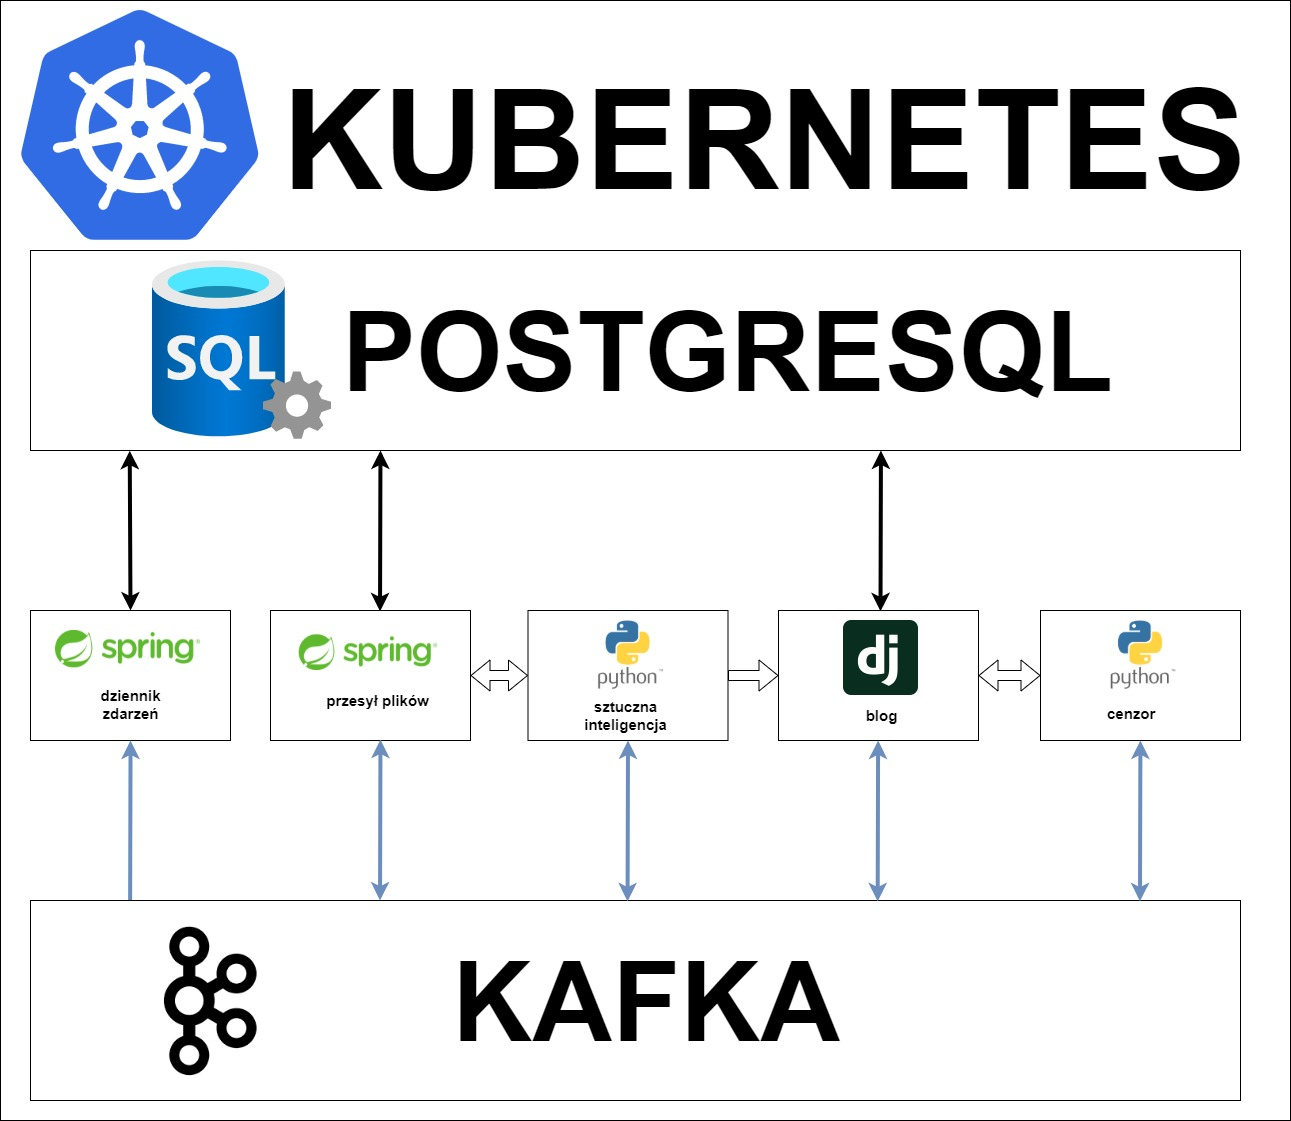
\includegraphics[width=16cm]{figures/diagram.jpg}
	\caption{Schemat implementowanego stosu aplikacji}
\label{Fig:schemat}
\end{figure}

Głównym mikroserwisem jest blog, serce całego stosu mikroserwisów napisane w języku \texttt{Python} z zastosowaniem frameworku \texttt{Django}. Udostępnia on funkcjonalności typowego bloga, czyli utworzenie konta użytkownika, tworzenie artykułów oraz dodawanie komentarzy. Do napisania cenzora (ang. \textit{censor}) również użyto języka \texttt{Python}. Przyjmuje on tekst w języku angielskim, sprawdza czy istnieją w nim słowa uważane za nieprzyzwoite, a następnie wysyła ten sam tekst z ocenzurowaną zawartością. Dziennik wydarzeń (ang. \textit{logs}) został napisany w \texttt{Javie} z wykorzystaniem frameworku \texttt{Spring Boot}. Odpowiada on za przyjęcie informacji o wydarzeniach mających miejsce w aplikacji i zapisaniu ich do bazy danych. Następną aplikacją, również napisaną w \texttt{Javie}, jest aplikacja przekazu plików (ang. \textit{fileuploader}), udostępniająca funkcjonalność zapisu plików do bazy danych. Ostatnią usługą jest mikroserwis sztucznej inteligencji(ang. \textit{ai}), prosta aplikacja w języku \texttt{Python} analizująca przesłane do niej zdjęcia w formacie \texttt{jpeg}. Wykrywa na tych zdjęciach twarze osób znajdujących się na nich, następnie umieszcza twarz w ramce, a na koniec oznacza płeć i kategorię wiekową wykrytych osób.

\subsubsection{Sposób implementacji}

Pracę nad implementacją zaczęto od zaplanowania sposobu działania mikroserwisów oraz zakres ich funkcjonalności.
Funkcjonalności mikroserwisów uzupełniają się nawzajem. Sposobem kierowania mikroserwisów jest choreografia\footnote{choreografia — wzorzec budowy mikroserwisów zakładający brak orkiestratora. Mikroserwisy same mają wiedzieć na jaki temat \texttt{kafki} wysłać wiadomość, z jakiego tematu ją pobrać i jak ją przetworzyć\cite{eventDrivenMicroservices}.} — mikroserwisy same w sobie wiedzą, który mikroserwis ma wykonać jakie połączenie do współpracy z innym mikroserwisem.

Kolejnym elementem przygotowującym do implementacji było utworzenie lokalnej instancji brokera \texttt{kafka} w oparciu o usługę przechowywania i udostępniania metadanych \texttt{Zookeeper} oraz instancji usługi bazy danych. Utworzono konfigurację środowiska programistycznego oraz bazy danych dla mikroserwisów. Następnie utworzono implementację mikroserwisów.

Wewnątrz blogu utworzono modele obiektów obsługujących bazę danych oraz skonfigurowano połączenie z lokalną instancją bazy danych \texttt{postgreSQL}. Aby udostępnić funkcjonalności strony internetowej z wykorzystaniem \texttt{API REST} utworzono serializatory przekształcające wcześniej utworzone modele na dane w postaci \texttt{JSON}.

Następnie dodano logikę biznesową działania aplikacji w widokach. Na koniec połączono logikę biznesową funkcjonalności z odpowiednimi punktami końcowymi i dodano połączenia z innymi mikroserwisami. Wewnątrz blogu nowo dodane artykuły i komentarze są domyślnie nieaktywne.

Dla mikroserwisu sztucznej inteligencji zmodyfikowano gotowy skrypt wykorzystujący bibliotekę \texttt{openCV} do zastosowania wyuczonej sieci neuronowej. Skrypt ten wykrywa twarze, płeć i kategorię wiekową wykrytych osób. Dzięki modyfikacji możliwe było użycie go jako mikroserwis. Następnie dodano do niego skrypt obsługujący połączenia z odpowiednimi mikroserwisami\cite{lib}.

Mikroserwisy dziennika zdarzeń oraz przekazu pliku posiadają podobną implementację. W obu serwisach utworzono odpowiednie byty oraz odpowiadające im repozytoria i dodano logikę biznesową. Następnie utworzono kontrolery udostępniajace odpowiednie \texttt{endpointy} logiki biznesowej oraz dodano konfigurację użycia brokera wiadomości.

Mikroserwis cenzurujący wykorzystuje bibliotekę \texttt{profanity-filter}\cite{pf} do wykrycia cenzurowalnych treści w wiadomości. Napisano logikę biznesową działania mikroserwisu, a następnie skonfigurowano logikę współpracy z innymi serwisami. Wewnątrz tego mikroserwisu przetestowano działanie dwóch bibliotek obsługujących komunikację z wybranym brokerem wiadomości.

\subsubsection{Komunikacja z mikroserwisami}

Komunikacja wewnątrz stosu mikroserwisów została zaimplementowana poprzez wykorzystanie \texttt{API REST} oraz wykorzystanie konsumentów i producentów w brokerze wiadomości.

Wybranym brokerem wiadomości jest \texttt{Apache Kafka}\cite{kafka} ze względu na jego popularność, wysokie zastosowanie przez wiodące firmy z rankingu \texttt{Fortune 100} oraz doświadczenie w jego zastosowaniu uzyskane podczas pracy zawodowej.

W mikroserwisach \texttt{springowych} do połączeń przy użyciu brokera wykorzystano bibliotekę \texttt{Spring Cloud Stream}. Jest to biblioteka pozwalająca na obsługę więcej niż jednego brokera identycznym kodem tworzenia producenta i konsumenta. Jedynymi elementami, które należy zmienić to dodanie odpowiedniej konfiguracji biblioteki oraz dodanie biblioteki wiążącej aplikację z brokerem.

Aplikacje w języku \texttt{Python} wykorzystują klienta\footnote{klientem w tym kontekście nazywany jest obiekt implementijący konsumenta tematu \texttt{kafki}.} \texttt{confluent-kafka-python}\cite{confluent} oraz \texttt{kafka-python}\cite{kafka-python}. W ramach sprawdzenia bibliotek utworzono dwie wersje mikroserwisu cenzorującego. W przypadku użycia \texttt{confluent-kafka-python} na podstawie przykładu z dokumentacji udało się utworzyć skrypt, który pozwala na odczytywanie wielu tematów, przez wielu konsumentów. W przypadku \texttt{kafka-python} niemożliwe było utworzenie dwóch aktywnych klientów w jednym skrypcie. Do uzyskania podobnych funkcjonalności wymagane byłoby uruchomienie dwóch aplikacji \texttt{Python} w ramach mikroserwisu.

\texttt{API REST} zostało wykorzystane w aplikacjach do komunikacji z użytkownikiem oraz przesyłania spodziewanych, większych porcji danych pomiędzy aplikacjami. Z powodu ograniczeń wielkości wiadomości, przy użyciu \texttt{kafki} wysyłane są tylko najważniejsze informacje. Broker \texttt{kafka} posiada wbudowaną konfigurację ograniczającą wiadomości do 1MB. Ograniczenie można zmienić, jednak nie jest to zalecane. W przypadku wysyłania większych wiadomości broker przestaje pracować wydajnie. Wiadomości wysyłane na broker są wysyłane i odbierane asynchronicznie. Wiadomość z tematu zostaje odczytana w chwili zapytania o odczyt z tematu przez grupę konsumencką — grupę, do której uczestnictwo określa, gdzie jej uczestnicy mają rozpocząć dalsze odczytywanie kolejnych wiadomości. Każda grupa konsumencka posiada własny indeks informujący o położeniu odczytanych wiadomości.

Do nazywania tematów wykorzystano angielską nazwę wydarzenia mającego miejsce w mikroserwisie. Zastosowanie takiej konwencji nazewniczej pozwala, na wielokrotne zastosowanie tego samego tematu w przyszłości przy tworzeniu nowych rozwiązań mających ten sam punkt wyjściowy rozpoczęcia wykonywania funkcji, którym jest wydarzenie biznesowe.

\subsubsection{Opis połączeń między aplikacjami}
Wewnątrz stosu mikroserwisów wszystkie mikroserwisy komunikują się z serwisem dziennika zdarzeń. Wysyłają do niego informację o wydarzeniach mających miejsce wewnątrz nich na określony temat \texttt{kafki}.

Mikroserwis przesyłu danych wysyła informację o zapisie nowych plików na temat \texttt{fileCreated}. Mikroserwis sztucznej inteligencji, który posiada konsumenta obserwującego ten temat odczytuje wiadomość, pobiera plik i na podstawie jego rozszerzenia decyduje o tym czy przetworzyć go, czy przejść do następnej wiadomości. W przypadku przetworzenia wysyła gotowy, przetworzony plik do blogu, który zapisuje go i udostępnia do przejrzenia oraz umieszczenia w artykule.

Kolejne interakcje przeprowadzane są przy dodawaniu lub modyfikacji artykułów i komentarzy. Blog po wykonaniu akcji wysyła informację z id obiektu na temat \texttt{articleSaved} lub \texttt{commentSaved}. Mikroserwis cenzurujący nasłuchujący te tematy odczytuje zawartość wiadomości, wykonuje zapytanie do blogu o odpowiedni obiekt, a następnie cenzuruje treśc obiektu. Po ocenzurowaniu zawartości wysyła kolejne zapytanie z treścią już ocenzurowaną, którą blog przyjmuje i zapisuje pod tym samym \texttt{id} obiektu ze zmodyfikowaną treścią i statusem aktywnym dla obiektu.

\subsection{Wprowadzenie konteneryzacji}
Kolejnym krokiem tworzenia prototypu, było wprowadzenie konteneryzacji utworzonych mikroserwisów. Wykonano je poprzez utworzenie szablonów obrazów zadeklarowanych w plikach \texttt{dockerfile} oraz definicję stosu w pliku \texttt{docker-compose.yaml}. Na koniec każdy obraz udostępniono w rejestrze \texttt{dockerhub}\cite{myhub}.

\subsubsection{Obrazy kontenerów}
Pierwszym krokiem wprowadzenia konteneryzacji było zapoznanie się z tematem oraz wybór obrazów wykorzystywanych w tworzeniu aplikacji. Do implementacji kafki wykorzystano gotowy stos \texttt{docker-compose} od \texttt{bitnami}\cite{bitnami}.

Sposób uruchomienia stosu \texttt{kafka}:
\begin{lstlisting}[breaklines]
cd kafka
docker-compose up -d
\end{lstlisting}
Powyższy, gotowy plik pozwala na ominięcie trudnej konfiguracji sieci między kontenerami. Następnie przetestowano działanie powyższej usługi z użyciem lokalnie uruchomionych aplikacji. Zachowały się identycznie jak w przypadku lokalnej \texttt{kafki},  którą w trakcie sprawdzania usługi wyłączono.

W ramach stosu aplikacji napisanych w jęzku \texttt{Python} zdecydowano się na wykorzystanie obrazów \texttt{,,python:3.8''} dla usługi cenzora \texttt{,,python:3''} dla blogu oraz \texttt{,,python:latest''} w ramach usługi sztucznej inteligencji. Powodem wyboru określonych wersji jest zachowanie odpowiednich kompatybilności z bibliotekami wykorzystywanymi w mikroserwisach.

Aplikacje \texttt{springowe} wykorzystują obraz \texttt{,,adoptopenjdk/openjdk11:alpine''}. Powodem wyboru wersji \texttt{alpine} jest minimalny rozmiar końcowy obrazu. Przykład definicji obrazu:
\begin{lstlisting}[breaklines]
FROM adoptopenjdk/openjdk11:alpine
\end{lstlisting}
Wewnątrz plików \texttt{dockerfile} zdefiniowano zmienne lokalne, przez które mikroserwisy komunikują się ze sobą. Przykład definicji zmiennej środowiskowej:
\begin{lstlisting}
ENV LOGGER_PORT = 8888
\end{lstlisting}
Następnie wykorzystano zmienne środowiskowe w odpowiednich miejscach aplikacji. Dla aplikacji \texttt{Python}:
\begin{lstlisting}
os.getenv('UPLOADER', "localhost:8999")
\end{lstlisting}
\texttt{Java}:
\begin{lstlisting}
${UPLOADER_PORT:8999}
\end{lstlisting}
W powyższych przykładach drugim parametrem jest wartość domyślna, dodana w celu zachowania wstecznej kompatybilności z uruchamianiem aplikacji w środowisku lokalnym bez użycia kontenerów.

Kolejnym krokiem wprowadzenia konteneryzacji było zdefiniowanie plików, które są wykorzystywane w obrazie. Do uruchomienia aplikacji napisanych w języku \texttt{Java} wymagane jest tylko posiadanie pliku ,,\texttt{.jar}'', plik uruchomieniowy został skopiowany z folderu \texttt{target} — miejsca, w którym menedżer pakietów \texttt{maven} instaluje aplikację \texttt{Spring Boot}.
\begin{lstlisting}
ARG JAR_FILE=target/*.jar
COPY ${JAR_FILE} logs.jar
\end{lstlisting}
Powyższe instrukcje wybierają położenie pliku ,,\texttt{.jar}'' poprzez zastosowanie wyrażenia regularnego. Określają one nazwę pliku i przypisują ten plik do zmiennej istniejącej tylko podczas budowania obrazu. Następnie dany plik zostaje skopiowany do ścieżki głównej w obrazie przy pomocy instrukcji \texttt{copy}. W przypadku usług \texttt{Python} kopiujemy całą zawartość folderu z kodem do ścieżki relatywnej \texttt{/code}, a następnie zmieniamy ścieżkę głównej obrazu na ten folder.

\begin{lstlisting}
WORKDIR /code
ADD . /code/ 
\end{lstlisting}


Do uruchomienia rozwiązań w języku \texttt{Python} wymagane są dodatkowe biblioteki umożliwiające uruchomienie kodu. Z tego powodu dodano linijki, które uruchamiają polecenia bezpośrednio w budowanym obrazie w kolejności wystąpienia. W tym przypadku instalowane są niezbędne biblioteki \texttt{Python} uzyskane przy pomocy menedżera pakietów \texttt{pip}. Następnie dla środowiska wykonywana jest aktualizacja reporytoriów linuxowych, aby móc zainstalować ręcznie kodeki i biblioteki systemowe:
\begin{lstlisting}
RUN pip install -r requirements.txt
RUN apt-get update
RUN apt-get install ffmpeg libsm6 libxext6  -y
\end{lstlisting}
Do uruchomiania programów w języku \texttt{Java} wykorzystano poniższe instrukcje:
\begin{lstlisting}
ENTRYPOINT ["java","-jar","/uploader.jar"]
\end{lstlisting}
Natomiast poniższe instrukcje uruchamiają aplikacje w języku \texttt{Python}:
\begin{lstlisting}
CMD ["python3", "confluent.py"] #censor
ENTRYPOINT ["python", "manage.py", "runserver", "0.0.0.0:8001"] #blog
\end{lstlisting}
Powyższe instrukcje wykonują polecenia z wiersza linii poleceń wewnątrz kontenera. Główną różnicą pomiędzy komendą \texttt{ENTRYPOINT} i \texttt{CMD} jest możliwość zmiany wartości parametrów dla \texttt{CMD}. \texttt{ENTRYPOINT} po dodaniu parametru przy wywołaniu dopisze go na koniec. Komenda \texttt{ENTRYPOINT} została użyta w szablonie obrazu dla klastra \texttt{kubernetes}. Aby umożliwić uruchomienie różnych wersji cenzora (\texttt{main.py}, \texttt{other.py}, \texttt{confluent.py}) wykorzystano komendę \texttt{CMD}, która umożliwia zmianę parametrów wywołania. Przykład użycia kontenera z komendą \texttt{CMD} z parametrem:
\begin{lstlisting}
sudo docker run [nazwa kontenera] main.py
\end{lstlisting}
W powyższej instrukcji do \texttt{nazwa kontenera} wpisuje się nazwę kontenera dla instancji uruchomionej usługi. Po wpisaniu nazwy kontenera aplikacji cenzor, powyższe polecenie zastąpiło \texttt{confluent.py} wartością \texttt{main.py} wykorzystującą inną bibliotekę \texttt{kafki}.

Dla blogu i aplikacji napisanych w \texttt{Javie} postanowiono nieumożliwienie zmiany wartości parametrów. Ze względu na możliwość przyszłego rozwoju mikroserwisu sztucznej inteligencji o uruchamianie innego algorytmu wykorzystując ten sam moduł i obraz \texttt{dockerowy} umożliwiono zmianę parametru.

Warto zaznaczyć, że skonteneryzowano również bazę danych. Utworzono plik \texttt{dockerfile} dla usługi postgres. W szablonie obrazu dodano dwie dodatkowe konfiguracje, skrypt inicjalizujący bazę danych w odpowiednim miejscu komendami:
\begin{lstlisting}
COPY init.sql /docker-entrypoint-initdb.d/
\end{lstlisting}
oraz udostępnienie dostępu do bazy danych z zewnętrznych adresów ip:
\begin{lstlisting}
RUN echo listen_addresses = '*' >> postgres.conf
\end{lstlisting}

Plik \texttt{init.sql} jest skryptem inicjalizującym konto użytkownika oraz bazy danych, napisanym w składni odpowiedniej dla \texttt{postgreSQL}. Obraz domyślny jest skonfigurowany tak, aby każdy plik ,,\texttt{.sql}'' znajdujący się w danym miejscu został uruchomiony przy inicjalizacji bazy danych.

Aby umożliwić sprawdzanie poprawności działania zmian w modelach obraz \texttt{dockerfile} nie zawiera definicji wolumenów. Jest to celowe działanie, ponieważ pozwala ono na sprawdzenie poprawności wykonywania skryptu inicjalizacyjnego przy każdym uruchomieniu.

W późniejszej części pracy wykonano implementację innego pliku obrazowego, odpowiedniego do wdrożenia w klaster \texttt{kubernetes}. W implementacji blogu w plikach dla \texttt{dockera} i \texttt{docker-compose} wykorzystano plik \texttt{localdockerfile}, a nie \texttt{dockerfile} jak pozostałe implementacje. Pod nazwą \texttt{dockerfile} istnieje plik używany przez konfigurację \texttt{kubernetes}.

Wszelkie ręczne budowania obrazu wymagają określenia nazwy pliku jak poniżej:
\begin{lstlisting}
docker build -f localdockerfile . -t blog
\end{lstlisting}
wewnątrz katalogu \verb|blog_app.|

Wykonano wielokrotne próby nawiązania połączenia między ręcznie uruchomionym kontenerem oraz usługą \texttt{kafki} uruchomioną poprzez \texttt{docker-compose}. W tym celu zbudowano obrazy komendami:
\begin{lstlisting}
cd blog_app
docker build -f localdockerfile . -t blog
\end{lstlisting}
Gdzie parametr ,,\texttt{-t}'' określał nazwę obrazu. Użycie komendy bez podania nazwy generowało domyślną wartość, której nie sposób zrozumieć. Przykład takiej nazwy:
\begin{lstlisting}[breaklines]
sha256:8ebc65f7c6f4b051b98fca7340f87b9ec8889bf071c3aa496d
d0118eba126031
\end{lstlisting}
Następnie utworzono sieć pomiędzy usługami
\begin{lstlisting}
docker network create microservices
\end{lstlisting}
oraz połączono do sieci kontenery dla istniejących usług \texttt{kafki} i \texttt{zookeepera}
\begin{lstlisting}
docker network connect microsevices kafka
docker network connect microservices zookeeper
\end{lstlisting}
i uruchomiono kontener połączony z siecią:
\begin{lstlisting}
docker run -p 8001:8001 -d --name blog --network microservices
...
\end{lstlisting}
Opcja ,,\texttt{-p}'' w powyższym przykładzie upublicznia porty wewnętrzne i zewnętrzne dla usługi.

Niestety nie udało się połączyć z usługą, pomimo utworzenia sieci pomiędzy nimi. Wiadomość ,,\texttt{no broker available}'' wewnątrz mikroserwisów informowała, że usługa blog uruchomiona ręcznie jako kontener nie mogła połączyć się z usługą uruchomioną w \texttt{docker-compose}. Po dłuższym zapoznaniu się z problemem głównie polegającym na przeglądaniu rozwiązań z forum programistycznego stack-overflow uznano, że połączenia pomiędzy pojedynczymi instancjami uruchomionymi przez \texttt{docker} na zewnątrz są wielkim problemem. Istnienie lepszego rozwiązania przy wykorzystaniu \texttt{docker-compose} sprawił, że postanowiłem nie poświęcić mu dłuższej uwagi.

\subsubsection{Stos kontenerów}
Następnie przygotowano plik \texttt{docker-compose.yaml} dla stosu kontenerów. Do pliku dodano wartości z importowanego wcześniej pliku \texttt{docker-compose.yaml} od \texttt{bitnami} oraz konfigurację każdego uruchamianego serwisu. Wewnątrz pliku zadeklarowano wersję deklaracji \texttt{docker-compose} oraz definicję serwisów:
\begin{lstlisting}
version: "3"
services:
  blog:
\end{lstlisting}
W powyższym przykładzie nazwa usługi — ,,\texttt{blog}'' określa nazwę wewnętrzną, po której można komunikować się z określoną usługą. Sieć wewnętrzna w ramach jednego pliku \texttt{docker-compose} zostaje utworzona automatycznie. Następnie zdefiniowano ścieżkę pliku \texttt{dockerfile}, na podstawie którego należy zbudować obraz usługi:
\begin{lstlisting}
    build: blog_app/.
\end{lstlisting}
Ścieżka pliku jest ścieżką względną pliku \texttt{docker-compose}. W przypadku braku tej wartości i istnieniu wartości dla parametru \texttt{image}, \texttt{docker} spróbuje pobrać obraz o podanej nazwie z rejestru \texttt{dockerhub}. Jeżeli wartość obrazu jest podana razem ze ścieżką budowania, zbudowany obraz otrzyma nazwę podaną jako parametr \texttt{image}.

Następnie skonfigurowano dostęp zewnętrzny do portów:
\begin{lstlisting}
    ports:
    - "9090:8001"
\end{lstlisting}
Po lewej stronie znajduje się informacja, jaki port ma być dostępny na zewnątrz. Po prawej, jaki port wewnętrzny jest mapowany. W powyższym przykładzie usługa była udostępniona wewnątrz kontenera na porcie ,,\texttt{8001}'', pozostałe serwisy mogą przez ten port komunikować się z danym serwisem. Na zewnątrz klient uzyskiwał do niej dostęp na porcie ,,\texttt{9090}''.

Kolejną, zadeklarowaną właściwością w pliku \texttt{docker-compose} było ponowne uruchamianie usługi w przypadku błędu. W utworzonym stosie istniały usługi zależne od innych. Blog, sztuczna inteligencja oraz censor wymagały pełnej inicjalizacji \texttt{kafki} i bazy danych. Dla nich wykorzystywano mechanizm ponownego uruchomienia usługi przy nieoczekiwanym zamknięciu.
\begin{lstlisting}
    restart: always
\end{lstlisting}
Następnie zadeklarowano nazwy obrazu wykorzystywanego w usługach oraz nazwy kontenerów, po których można się do nich odwoływać. Przykład poniżej:
\begin{lstlisting}
    container_name: blog
    image: bfinger1997/blog
\end{lstlisting}
Kolejnym elementem, który wprowadzono do stosu były wolumeny:
\begin{lstlisting}
  volumes:
    - ./database:/var/lib/postgresql/data
\end{lstlisting}
Pozwalały one na mapowanie położenia zapisywanych plików w kontenerze na dysku. Udostępniło to wprowadzenie persystencji danych\footnote{persystencja danych — trwałość danych pomiędzy uruchomieniami programu poprzez zapisywanie ich w osobnym miejscu, na przykład w bazie danych lub na nośniku fizycznym}, które w przypadku kontenerów są ulotne. Po wykonaniu tej części pracy zdecydowano się na zakomentowanie wolumenów, na rzecz wykorzystania pliku \texttt{docker-compose} przy wdrażaniu serwisów na klaster \texttt{kubernetes}. Istnienie wolumenów mogłoby doprowadzić do nieoczekiwanego stanu początkowego, przez który aplikacje nie mogłyby wystartować wewnątrz klastra.

Następnie wprowadzono zmienne lokalne poprzez zastosowanie plików ,,\texttt{.env}'' oraz listy \texttt{environment}:
\begin{lstlisting}
    env_file:
      - blog_app/blog.env #blog
   	...
   	environment: #postgres
      - POSTGRES_PASSWORD=qwe123
      - POSTGRES_DB=postgres
\end{lstlisting}
Pozwalało to na dodanie oraz nadpisanie wartości zmiennych środowiskowych. Właściwości w pliku ,,\texttt{.env}'' posiadają priorytet wyższy nad właściwościami wpisanymi w plik \texttt{dockerfile} — nadpisują je. Zmienne z listy \texttt{environment} posiadają najwyższy priorytet.

Następnie przetestowano możliwość zmiany położenia folderu głównego:
\begin{lstlisting}
    working_dir: /code/tets
\end{lstlisting}
W interakatywnym połączeniu z kontenerem potwierdzono zmianę właściwości:
\begin{lstlisting}
PS C:\Users\bartek\Documents\paluch bartlomiej praca dyplomowa>docker exec -it censor bash
root@1b203d6b28c7:/code/tets#
\end{lstlisting}
Zmiana położenia jest przydatna, jeżeli posiadamy te różne pliki, których funkcjonalności są zależnymi od położenia. Dla przykładu w położeniach ,,\texttt{code}'' i ,,\texttt{code/tets}'' komenda
\begin{lstlisting}
    python confluent.py
\end{lstlisting}
będzie działać różnie w zależności od tego, w którym folderze się znajduje.
W folderze, w którym nie występuje plik wpisanie nieprawidłowej wartości wskazywało, że plik \texttt{confluent.py} nie istnieje.

Następnie w usłudze sztucznej inteligencji wykorzystano właściwość replikacji:
\begin{lstlisting}
    deploy:
      replicas: 10
\end{lstlisting}
Pozwoliła ona na wprowadzenie dwóch kontenerów korzystających z tego samego obrazu. Warto podkreślić, że nie jest to doskonałe rozwiązanie w przypadku \texttt{docker-compose}. Wymagało ono wyłączenia mapowania portów. Dodatkowo nie można kontrolować, która uruchomiona instancja aktualnie obsługuje daną wiadomość, czy jest to pierwsza, czy piąta. Na podstawie logów \texttt{kafki} potwierdzono, że grupę obsługuje 10 instancji. 
\begin{lstlisting}
Stabilized group ai generation 31 (__consumer_offsets-12) with 10 members 
(kafka.coordinator.group.GroupCoordinator)
\end{lstlisting}

Dodano również obsługę zależności. Usługa nie zostanie uruchomiona, jeżeli inna usługa nie jest uruchomiona:
\begin{lstlisting}
    depends_on:
      - postgres
      - kafka
      - zookeeper
\end{lstlisting}
Powyższy serwis, zawierający daną konfigurację nie podejmował próby uruchomienia, jeżeli serwisy, od których był zależny, nie zostały uruchomione. Test wykonano uruchamiając bazę danych \texttt{postgres} jako pojedynczy obraz z identyczną nazwą kontenera. \texttt{Postgres} nie został uruchomiony ze względu na konflikt nazw. Dla usług zależnych od niego nie dokonano próby ich uruchomienia. 

Na koniec zdefiniowano komendy uruchomienia dla migracji bazy danych i blogu:
\begin{lstlisting}
command: "python manage.py migrate --noinput"
\end{lstlisting}
Oprócz wykonania komend zawartych w pliku \texttt{dockerfile} podczas budowania obrazu powyższa komenda zostaje wykonana dodatkowo po zbudowaniu obrazu.

Ostatnim krokiem było dodanie obrazów do repozytoriów. Wykonano to poprzez zalogowanie do usługi rejestru \texttt{dockerhub} na stronie usługi\cite{hub}, dodanie repozytoriów, a następnie zalogowanie w linii poleceń do rejestru \texttt{dockerhub} i przesłanie odpowiednio zbudowanych obrazów do repozytoriów. Poniższe komendy wykonały budowę i dodanie obrazu do istniejącego repozytorium, na którym wcześniej użytkownik został zalogowany:
\begin{lstlisting}
cd censor
build . -t bfinger1997/censor
docker push bfinger1997/censor
\end{lstlisting}
Nazwy wszystkich obrazów i skrócone komendy znajdują się w instrukcji załączonej z tą pracą.

\subsection{Wdrożenie usług skonteneryzowanych}
Kolejnym etapem było przygotowanie plików wdrożeniowych na klaster lokalny oraz publiczny. Ze względu, że publiczne usługi \texttt{kubernetes} są płatne pierwszym środowiskiem testowym, jest środowisko lokalne.

\subsubsection{Klaster lokalny}
Na rzecz środowiska lokalnego wykorzystano klaster wbudowany w \texttt{docker-desktop}. Pozwolił on na pominięcie kilku etapów konfiguracji środowiska oraz instalacji dodatkowych narzędzi.

W ramach wdrożenia klastra lokalnego przygotowano odpowiednie dla usług pliki ,,\texttt{deployment.yaml}''. Pliki te zawierają definicję zasobów klastrowych.
Pomiędzy definicją każdego zasobu znajduje się linia separująca definicję zasobów:
\begin{lstlisting}
---
\end{lstlisting}

W ramach każdej usługi przygotowano mapę konfiguracyjną ze zmiennymi środowiskowymi:
\begin{lstlisting}
apiVersion: v1
kind: ConfigMap
metadata:
  name: ai-config
  labels:
    app: ai
data:
  UPLOADER: http://uploader:8999
  KAFKA_HOST: kafka:9092
  BLOG: http://blog:8001/api
\end{lstlisting}
Mapa ta zawiera informację o obsługiwanej wersji konfiguracyjnego \texttt{API}. W przypadku aplikacji w tym projekcie wszystkie mapy utworzono w wersji ,,\texttt{v1}''.
Parametr \texttt{kind} opisuje typ zasobu. Następnie w treści metadanych umieszczona została nazwa zasobu oraz etykieta informująca jakiej aplikacji dotyczy dana mapa konfiguracyjna.
W części \texttt{data} umieszczone są wartości zmiennych środowiskowych.

Następnym zasobem opisanym w plikach był \texttt{deployment} — wdrożenie aplikacji.
\begin{lstlisting}
apiVersion: apps/v1
kind: Deployment
metadata:
  name: ai
spec:
  selector:
    matchLabels:
      app: ai
  replicas: 2
  template:
    metadata:
      labels:
        app: ai
    spec:
      containers:
        - name: ai
          image: bfinger1997/ai
          imagePullPolicy: IfNotPresent
          envFrom:
            - configMapRef:
                name: ai-config
\end{lstlisting}
Wykorzystano wersję \texttt{API} ,,\texttt{apps/v1}''. Wewnątrz elementu \texttt{spec} umieszczono selektor \texttt{PmatchLabels} przyporządkowujący etykiety do danego zasobu. Następnie parametr \texttt{replicas} zawiera docelową liczbę replik — instancji \texttt{podów} wdrażanego zasobu.

Następna właściwość \texttt{template} określa szablon opisujący wdrażaną aplikację. \texttt{Metadata} definiuje etykietę zasobu. Ta etykieta musi się zgadzać z wartością wskazywaną w selektorze dopasowania etykiety.
Fragment szablonu \texttt{spec} zawiera opis wykorzystywanych kontenerów. Znajdują się tutaj właściwości takie jak nazwa kontenera, nazwa wykorzystywanego obrazu, zasada ściągania obrazów oraz przypisanie mapy konfiguracyjnej jako źródło zmiennych środowiskowych w \texttt{podach}.
W przypadku mojej konfiguracji umieszczono odniesienie do obrazów z repozytoriów w \texttt{dockerhub}. Zasada pobierania \texttt{IfNotPresent} pobierze nowy obraz tylko i wyłącznie, jeżeli w rejestrze lokalnym nie istnieje obraz odpowiadający o nazwie podanego obrazu. 

W przypadku lokalnego środowiska zalecane jest ustawienie opcji \texttt{Never}, spowoduje to utworzenie i uruchomienie \texttt{podów} tylko i wyłącznie na podstawie obrazów w lokalnym rejestrze, a jeżeli te nie będą istnieć, to wdrożenie będzie oczekiwać, aż taki obraz zostanie dostarczony lokalnie. Aby umożliwić pominięcie procesu tworzenia własnych obrazów i repozytoriów, zdecydowano się wykorzystać zasadę \texttt{IfNotPresent}.
Dodatkowo wewnątrz usług wymagających skorzystania z wolumenów dodano poniższe wartości:
\begin{lstlisting}
   envFrom:
   ...
   volumeMounts:
    - mountPath: /var/lib/postgresql/data
      name: postgres-volume-storage
      readOnly: false
\end{lstlisting}
Wartości te określają w jakim miejscu należy zamontować wolumen w ramach położenia kontenera. W powyższym przykładzie użyte zostały wartości, które pozwalają na utrwalenie zawartości bazy danych.

Niektóre usługi wymagały udostępnienia portów zewnętrznym odbiorcom. W ramach wdrożenia utworzono serwisy \texttt{kubernetesowe}:
\begin{lstlisting}
apiVersion: v1
kind: Service
metadata:
  name: uploader
  labels:
    app: uploader
spec:
  type: NodePort
  ports:
    - port: 8999
  selector:
    app: uploader
\end{lstlisting}
Powyżej wyróżniono typ usługi — \texttt{NodePort}. Określono również port, który ma być otwarty z naszej aplikacji na świat. Na \texttt{NodePort} zdecydowano się ze względu na to, że \texttt{kubernetes} wewnątrz \texttt{KIND} jest klastrem jednowęzłowym.

Kolejnym zadeklarowanym zasobem była klasa przechowywania. Każda implementacja przechowywania trwałych wolumenów wymaga posiadania klasy przechowywania.

\begin{lstlisting}
apiVersion: storage.k8s.io/v1
kind: StorageClass
metadata:
  name: localstorage
provisioner: docker.io/hostpath
volumeBindingMode: Immediate
reclaimPolicy: Delete
allowVolumeExpansion: True
\end{lstlisting}

W przypadku \texttt{KIND} dostawcą implementacji lokalnego przechowywania wolumenu jest ,,\texttt{docker.io/hostpath}''. Ze względu na brak implementacji wdrożeń zaplanowanych czasowo ustawiono tryb wiązania wolumenu na \texttt{Immediate} -  natychmiastowe przypisanie żądania do zasobu, jeżeli jest to możliwe. Dodatkowo, w przypadku konieczności przechowywania większej ilości danych podczas testu ustawiono automatyczne zwiększanie wolumenu. Jako że brak miejsca powoduje niemal natychmiastowy paraliż stosu aplikacji, postanowiono nie pozwolić na taką sytuację. W związku z poprzednią decyzją, aby zachować miejsce na dysku oraz zapewnić, że olbrzymie wolumeny nie są przechowywane po usunięciu usługi, zastosowano zasadę odzysku \texttt{Delete}. Oznacza to, że w przypadku usunięcia aplikacji, zasób również automatycznie zostanie usunięty. W przypadku wdrożenia rozwiązania w chmurę publiczną, co wykonano później, pozwoliło to dodatkowo na uniknięcie sytuacji, gdzie opłacamy dostęp do olbrzymiej przestrzeni dyskowej, która nie jest wykorzystywana.

Kolejnym etapem wdrożenia było utworzenie samych wolumenów i przypisań do nich żądań. Tworzenie wolumenu:  
 \begin{lstlisting}
 apiVersion: v1
kind: PersistentVolume
metadata:
  name: blog-storage
spec:
  storageClassName: blogstorage
  capacity:
    storage: 2Gi
  accessModes:
    - ReadWriteMany
  persistentVolumeReclaimPolicy: Retain
  hostPath:
    path: "/C/blog"
    type: DirectoryOrCreate
 \end{lstlisting} 
Tworzenie przypisania:
  \begin{lstlisting}
 apiVersion: v1
kind: PersistentVolumeClaim
metadata:
  name: blog-persistent-volume-claim
spec:
  storageClassName: blogstorage
  accessModes:
    - ReadWriteMany
  resources:
    requests:
      storage: 2Gi
 \end{lstlisting} 
Ze względu na podobieństwo obu tych opisów wdrożeń, postanowiono opisać je razem.  Aby przypisanie zostało nadane, zarówno żądanie, jak i wolumen musiały być tej samej klasy, zasady odzysku oraz sposobu dostępu. Przy określeniu zasady automatycznego powiększania wolumenów dla klasy przechowywania, w przypadku gdy nie istnieje wolumen spełniający właściwości żądania, zostanie on automatycznie utworzony. W przeciwnym wypadku, gdy nie jest ustawione automatyczne powiększanie, żądanie będzie oczekiwać na pojawienie się wolumenu, który może je obsłużyć, jednak dopóki takowy się nie znajdzie, usługa nie zostanie uruchomiona.

Tryb dostępu ustawiono na wielokrotne połączenie zapisu/odczytu. Pozwoliło to na połączenie się wielu \texttt{podów} występujących w ramach wdrożenia z tym samym wolumenem. Dodatkowo dodano ścieżkę hosta, która dla implementacji przechowywania danych w pliku lub katalogu emuluje zachowanie magazynu sieciowego.
 
Do wdrożenia brokera kafka wykorzystano gotowy plik \texttt{helm}\footnote{plik helm — plik w formacie \texttt{yaml} zawierający szablon w języku Go upraszczający konfigurację wdrożenia. Wymaga instalacji programu \texttt{helm}} od \texttt{bitnami}\cite{helm} wdrażający zookeepera oraz kafkę wewnątrz klastra.
Jego aplikacja to instalacja narzędzia helm i wykonanie 3 linijek, tak aby wprowadzić w pełni funkcjonalny broker w klaster. Pozwoliło to na ominięcie trudnej dla osób niedoświadczonych konfiguracji brokera.
Instrukcje instalacyjne znajdują się w załączonej instrukcji instalacji. Zapoznano się z innymi możliwymi gotowymi stosami \texttt{kafka} dla klastra \texttt{kubernetes}, takimi jak rozwiązanie \texttt{Strimzi}. Pełen stos obsługujący kafkę od \texttt{Strimzi} posiada wbudowane systemy ochrony, które wymagają konfiguracji uwierzytelniania, obsługi kluczy oraz znajomości wielu aspektów produkcyjnych. Na podstawie doświadczenia z pracy zdecydowano, że rozwiązanie to jest zbyt obszerne i trudne w implementacji na rzecz tej pracy inżynierskiej, a jego użycie wprowadziłoby niepotrzebny chaos do implementacji.

\subsubsection{Klaster publiczny}

W ramach wdrożenia w klaster publiczny jako dostawcę wdrożenia wybrano rozwiązanie \texttt{Azure Kubernetes Service}. Jest to usługa, wybrana ze względu na znajomość autora pracy inżynierskiej ze stosem rozwiązań \texttt{Microsoft}, w ramach programu \texttt{Microsoft Imagine} udostępnionego przez uczelnię. Pierwszy miesiąc korzystania z usług chmurowych w \texttt{Azure} był w pełni darmowy do określonej kwoty. Kwota przyznana była w pełni wystarczająca do utworzenia oraz przetestowania wdrożenia.

W ramach przygotowania do wdrożenia usług w \texttt{AKS} utworzono klaster publiczny. Następnie zalogowano się do klastra, dzięki czemu uzyskano kontekst klastra - plik konfiguracyjny pozwalający na komunikację z nim przez zastosowanie narzędzia linii poleceń \texttt{kubectl}. Jest to narzędzie służące do wydawania poleceń w klastrze. Po utworzeniu i połączeniu się z klastrem wypróbowano wcześniej utworzone pliki wdrożeń. Aplikacja nie działała prawidłowo, ze względu na występujące problemy konfiguracyjne powstałe przez konflikty implementacyjne. Ze względu na to, odpowiednio zmodyfikowano pliki wdrożeniowe.
W związku z wykorzystywaniem \texttt{microsoftowego} rozwiązania \texttt{kubernetes} należy dostosować klasę przechowywania do klasy implementowanej w usłudze \texttt{AKS}. Zdecydowano się na wykorzystanie jednej z domyślnych klasy przechowywania \texttt{azurefile}. Jest ona zupełnie wystarczająca do obsługi tego projektu. Dodatkowo usunięto definicję \texttt{PersistentVolume}, jest ona niepotrzebna, ponieważ \texttt{AKS} automatycznie tworzy definicję \texttt{PersistentVolume} jeżeli posiada zdefiniowany \texttt{PersistentVolumeClaim}. Klaster automatycznie stworzy wymagany wolumen przy utworzeniu żądania.
  \begin{lstlisting}
apiVersion: v1
kind: PersistentVolumeClaim
metadata:
  name: blog-persistent-volume-claim
spec:
  storageClassName: azurefile
  accessModes:
    - ReadWriteMany
  resources:
    requests:
      storage: 2Gi
 \end{lstlisting}
Ze względu na to, że \texttt{AKS} udostępnia wiele węzłów, których liczba może wzrastać i maleć w zależności od obciążenia klastra, zadecydowano o zmianie typów serwisów na równoważnik obciążenia. Dzięki temu ruch do naszych usług zostanie rozesłany na wiele węzłów, a aplikacja będzie działać równie sprawnie, jak przy mniejszym obciążeniu, aż do osiągnięcia limitu liczby węzłów.
\begin{lstlisting}
apiVersion: v1
kind: Service
metadata:
  name: blog
  labels:
    app: blog
spec:
  type: LoadBalancer
  ports:
  - port: 8001
  selector:
    app: blog
 \end{lstlisting}
Po utworzeniu wszystkich plików wdrożeniowych wykonano instalację w klastrze \texttt{AKS}. Sposób instalacji w celu wykonania własnych testów został opisany w instrukcji, załączonej razem z kodem źródłowym.

W przypadku bazy danych zauważono niemożliwość wprowadzenia obrazu na wolumen typu \texttt{azurefile}. Związane jest to ze sposobem implementacji inicjalizacji \texttt{postgres}, oraz implementacji \texttt{azurefile}. \texttt{Azurefile} w implementacji jest oparty o serwer \texttt{SMB}, który pozwala na wprowadzenie praw własności oraz właściwości dostępu do całego serwera. Inicjalizacja \texttt{postgres} potrzebuje nadpisania prawa pojedynczego katalogu, co jest niewspierane przez serwer \texttt{SMB}. Z tego powodu użyto poniższe wartości:

  \begin{lstlisting}
apiVersion: v1
kind: PersistentVolumeClaim
metadata:
  name: database-persistent-volume-claim
spec:
  storageClassName: default
  accessModes:
    - ReadWriteOnce
  resources:
    requests:
      storage: 2Gi
 \end{lstlisting}
 
 Efektem zmiany typu dostępu jest to, że każdy wdrożony \texttt{pod} będzie posiadał własny wolumen, przez co umożliwia wdrożenie wielu \texttt{podów} bazy danych. Nie jest to dobre rozwiazanie, dlaczego opisano później w pracy w opisie zastosowań.
\subsection{Efekt działania wdrożonej aplikacji}
Następnie wykonano i dodano poniższe zdjęcia, ukazujące działanie aplikacji. Pomiędzy wykonaniem niektórych zdjęć miały miejsce testy elementów aplikacji, które wymagały przeinstalowania klastra. Z tego powodu adresy \texttt{IP} w przeglądarce nie zgadzają się na kilku zdjęciach. \begin{figure}[ht]
	\centering
	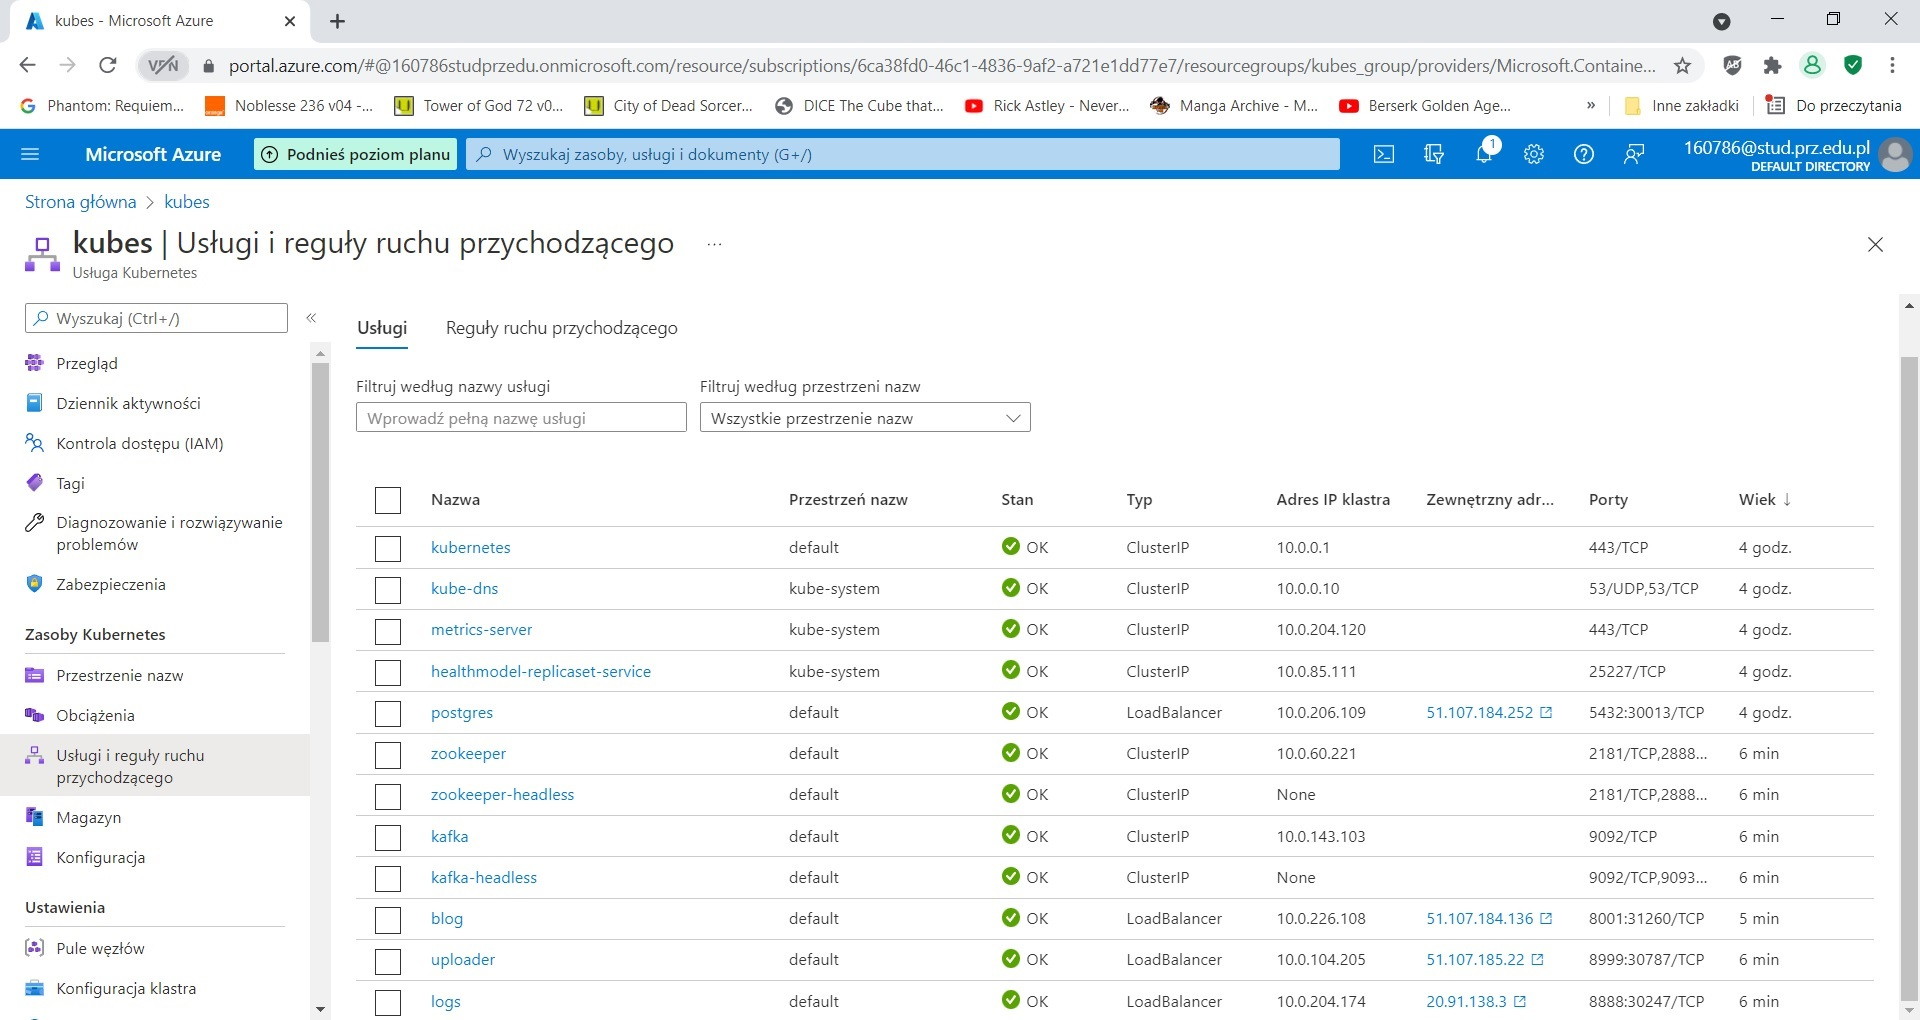
\includegraphics[width=11cm]{figures/klaster.jpg}
	\caption{Wdrożony klaster}
\label{Fig:cluster}
\end{figure}

Klaster został wdrożony w publicznej chmurze \texttt{Azure}. Rysunek \ref{Fig:cluster} ukazuje stronę w \texttt{AKS} zawierającą spis serwisów, które zawierała adresy dostępu do strony oraz porty, które zostały upublicznione.
Następny rysunek \ref{Fig:send} ukazuje żądanie, które zostało wysłane do serwisu przesyłu plików wraz z jego zawartością. W zawartości żądania wysłano zdjęcie do przetworzenia.
\begin{figure}[ht]
	\centering
	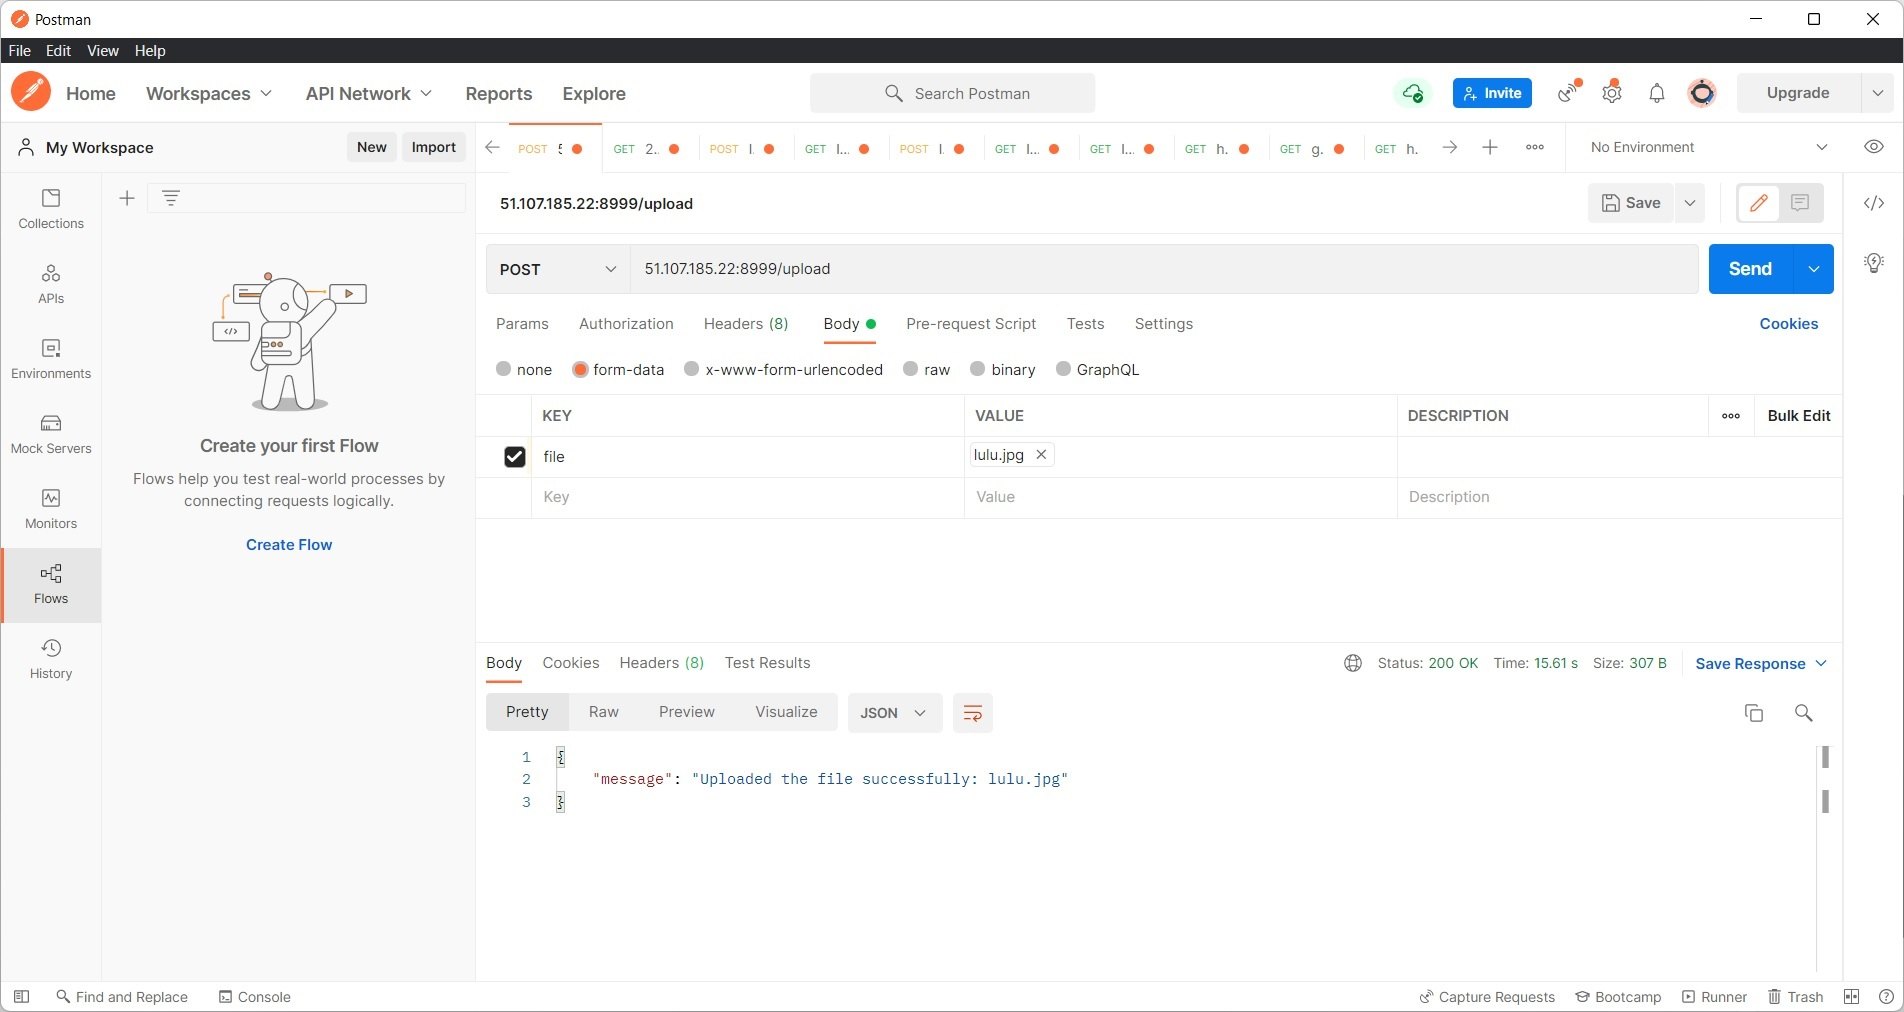
\includegraphics[width=11cm]{figures/send.jpg}
	\caption{Wysłanie i efekt żądania do przesyłu plików}
\label{Fig:send}
\end{figure}

Po wykonaniu żądania sprawdzono czy, plik na pewno został przyjęty przez serwis. Widoczne jest to na rysunku \ref{Fig:download}.
\begin{figure}[ht]
	\centering
	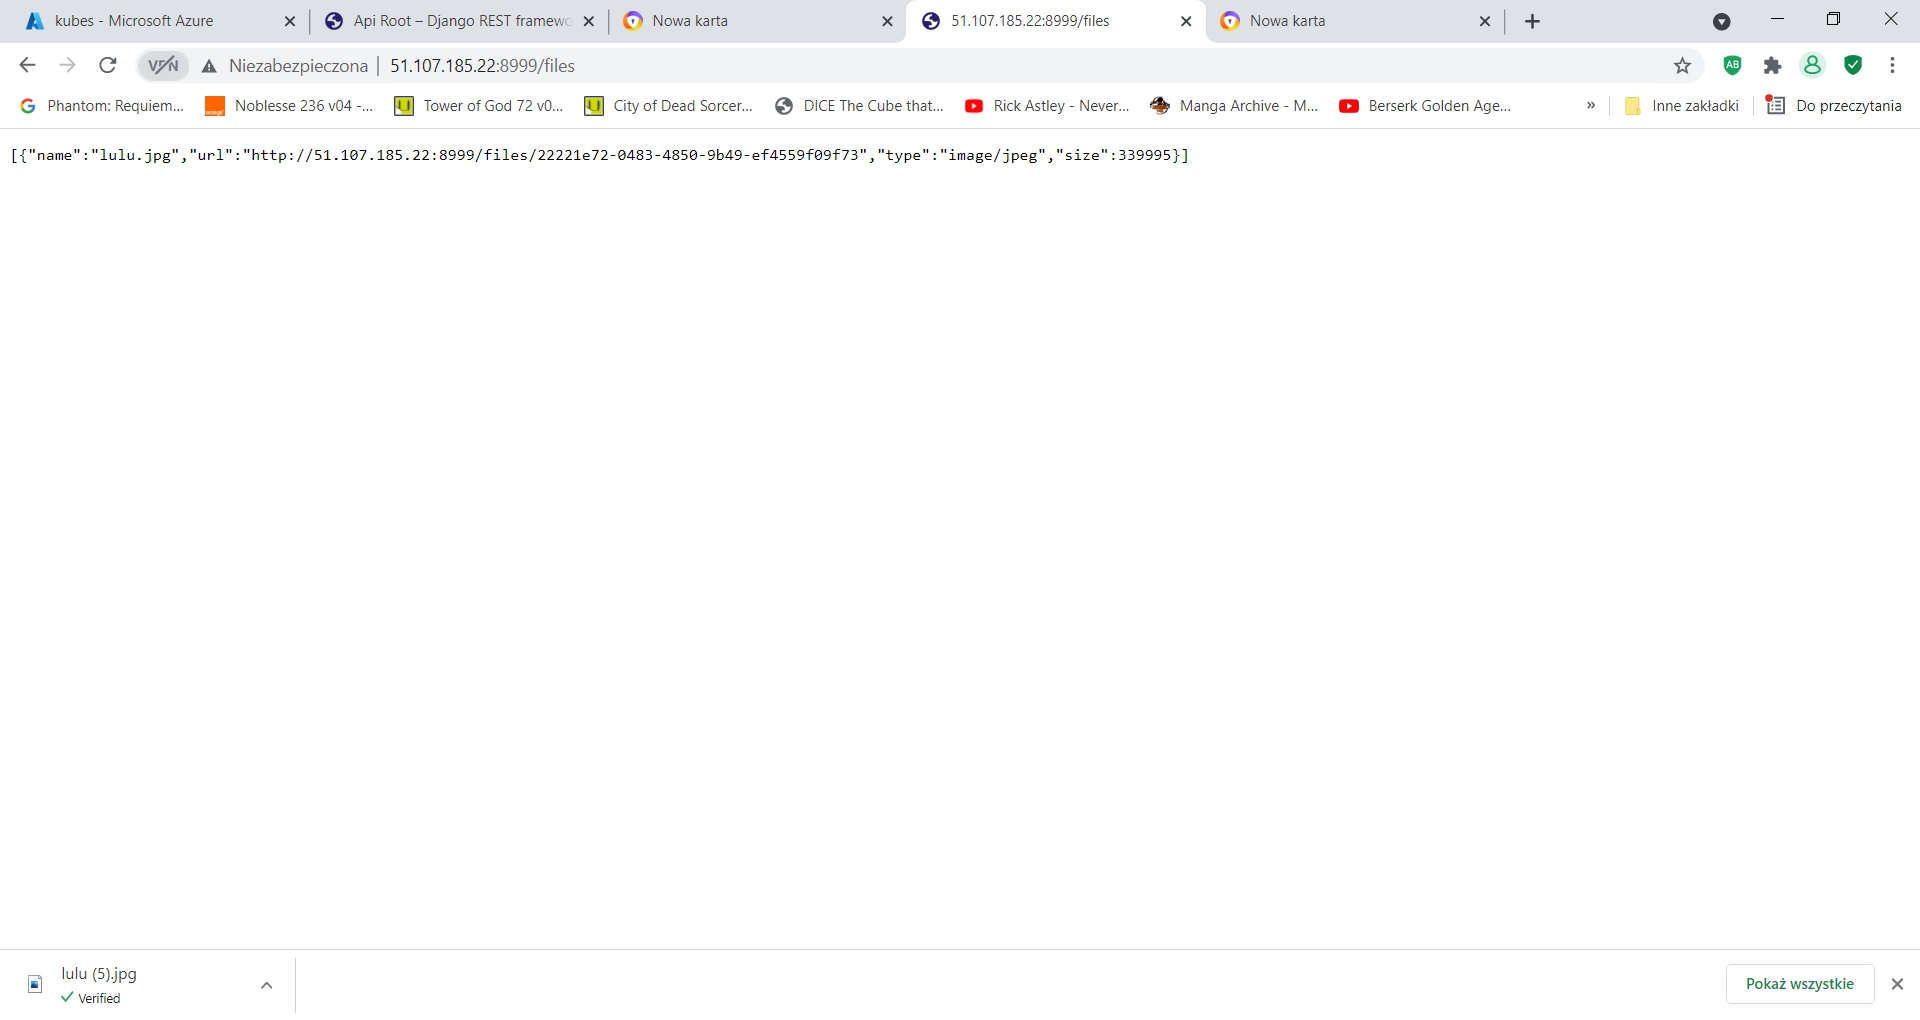
\includegraphics[width=11cm]{figures/download.jpg}
	\caption{Efekt żądania przesłania pliku}
\label{Fig:download}
\end{figure}

Po wysłaniu pliku sprawdzono, czy blog otrzymał go zgodnie z założeniem. Rysunek \ref{Fig:blog1} ukazuje efekt. Na rysunku \ref{Fig:blog} uwidoczniono efekt pracy serwisu sztucznej inteligencji.
\begin{figure}[ht]
	\centering
	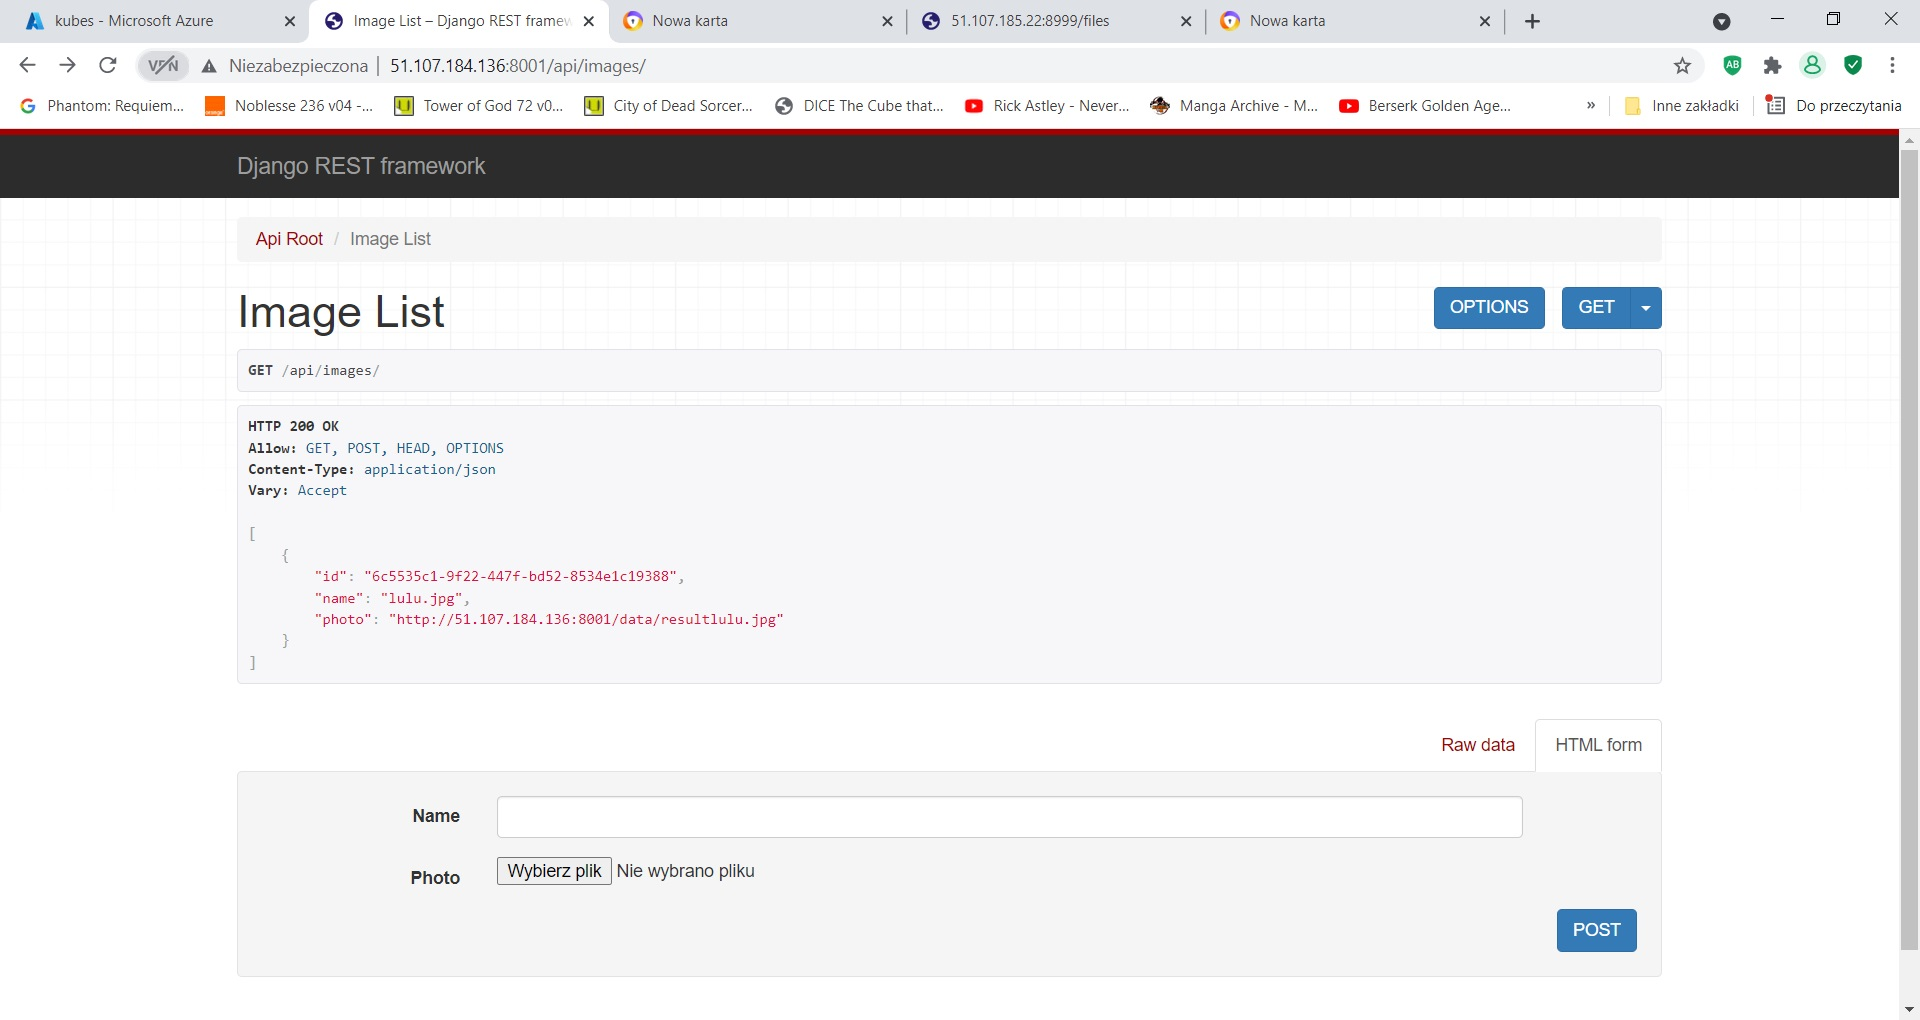
\includegraphics[width=11cm]{figures/blog1.jpg}
	\caption{Lista zdjęć na blogu}
\label{Fig:blog1}
\end{figure}

\begin{figure}[ht]
	\centering
	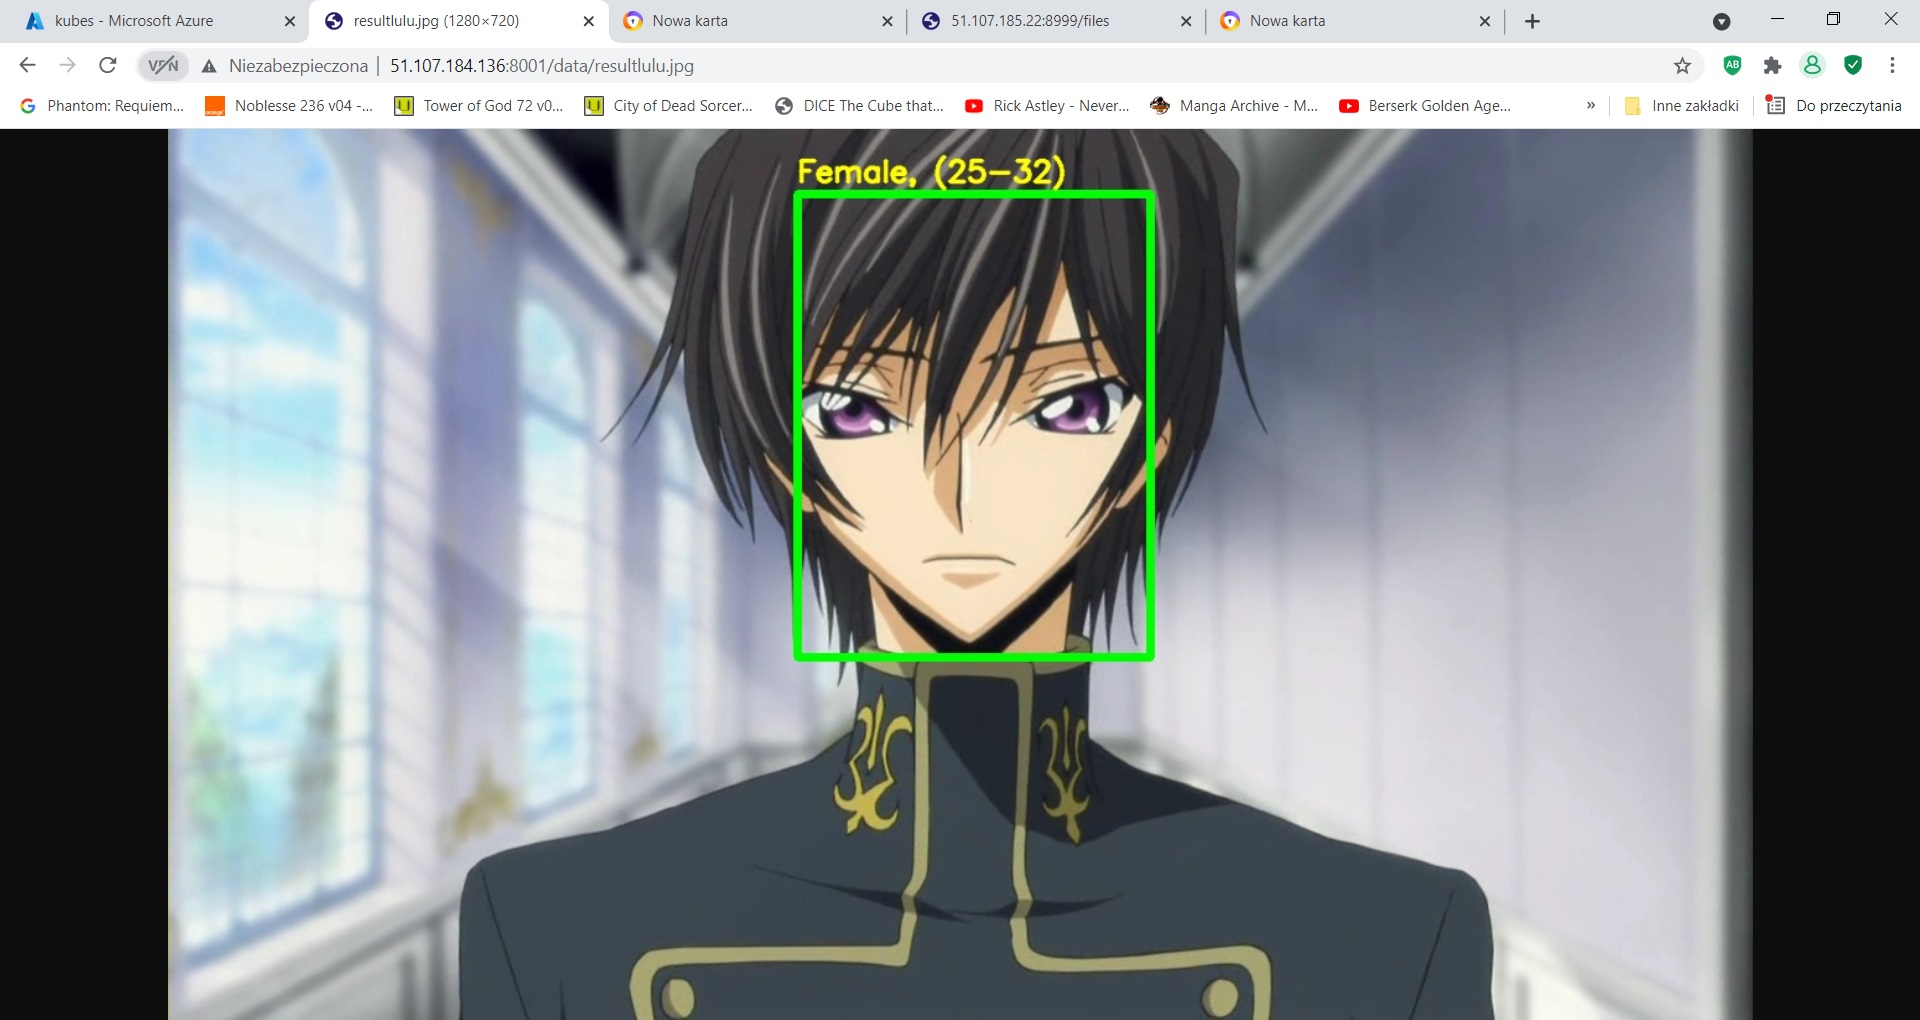
\includegraphics[width=11cm]{figures/blog.jpg}
	\caption{Zawartość zdjęć blogu}
\label{Fig:blog}
\end{figure}
Następnie sprawdzono możliwości cenzurowania przy dodawaniu artykułu. Rysunek \ref{Fig:blog2} zawiera wysłany, cenzuralny tekst. Rysunek \ref{Fig:blog3} ukazuje, że tekst został ocenzurowany oraz zaakceptowany.
\begin{figure}[ht]
	\centering
	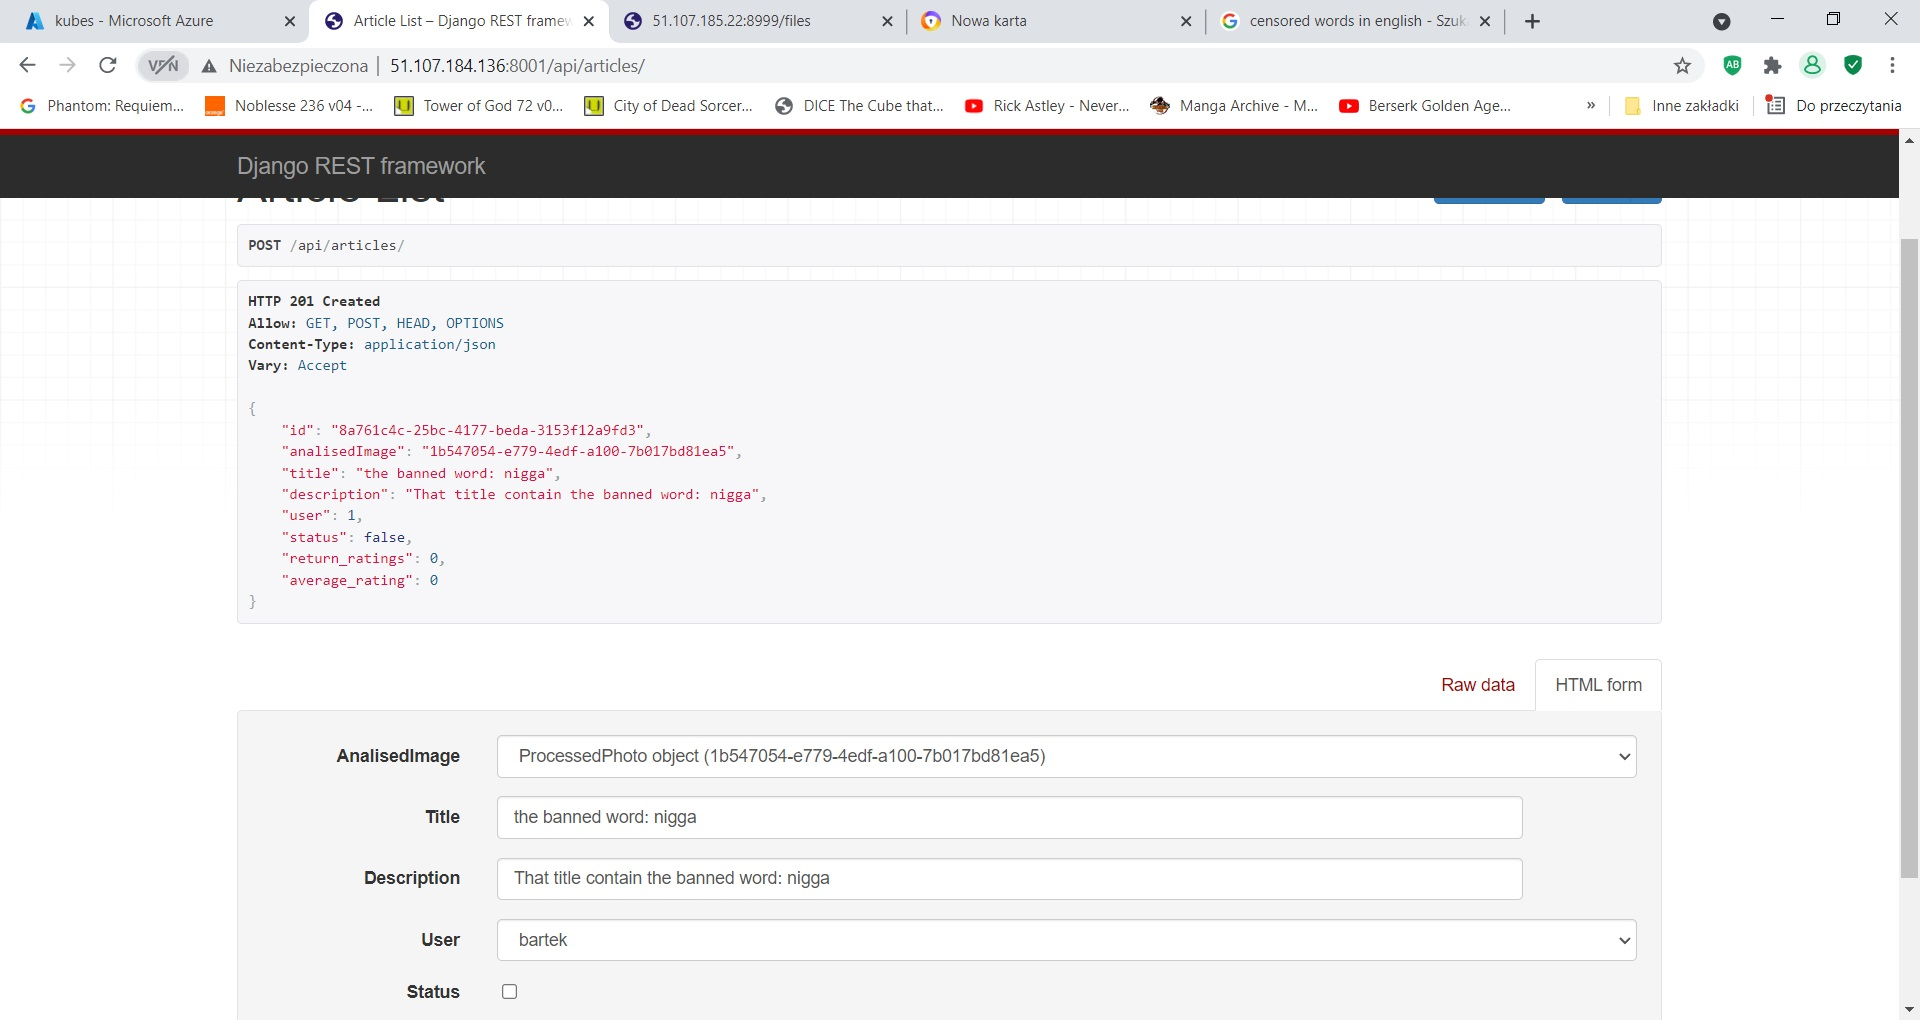
\includegraphics[width=11cm]{figures/blog2.jpg}
	\caption{Tworzony artykuł}
\label{Fig:blog2}
\end{figure}
\begin{figure}[ht]
	\centering
	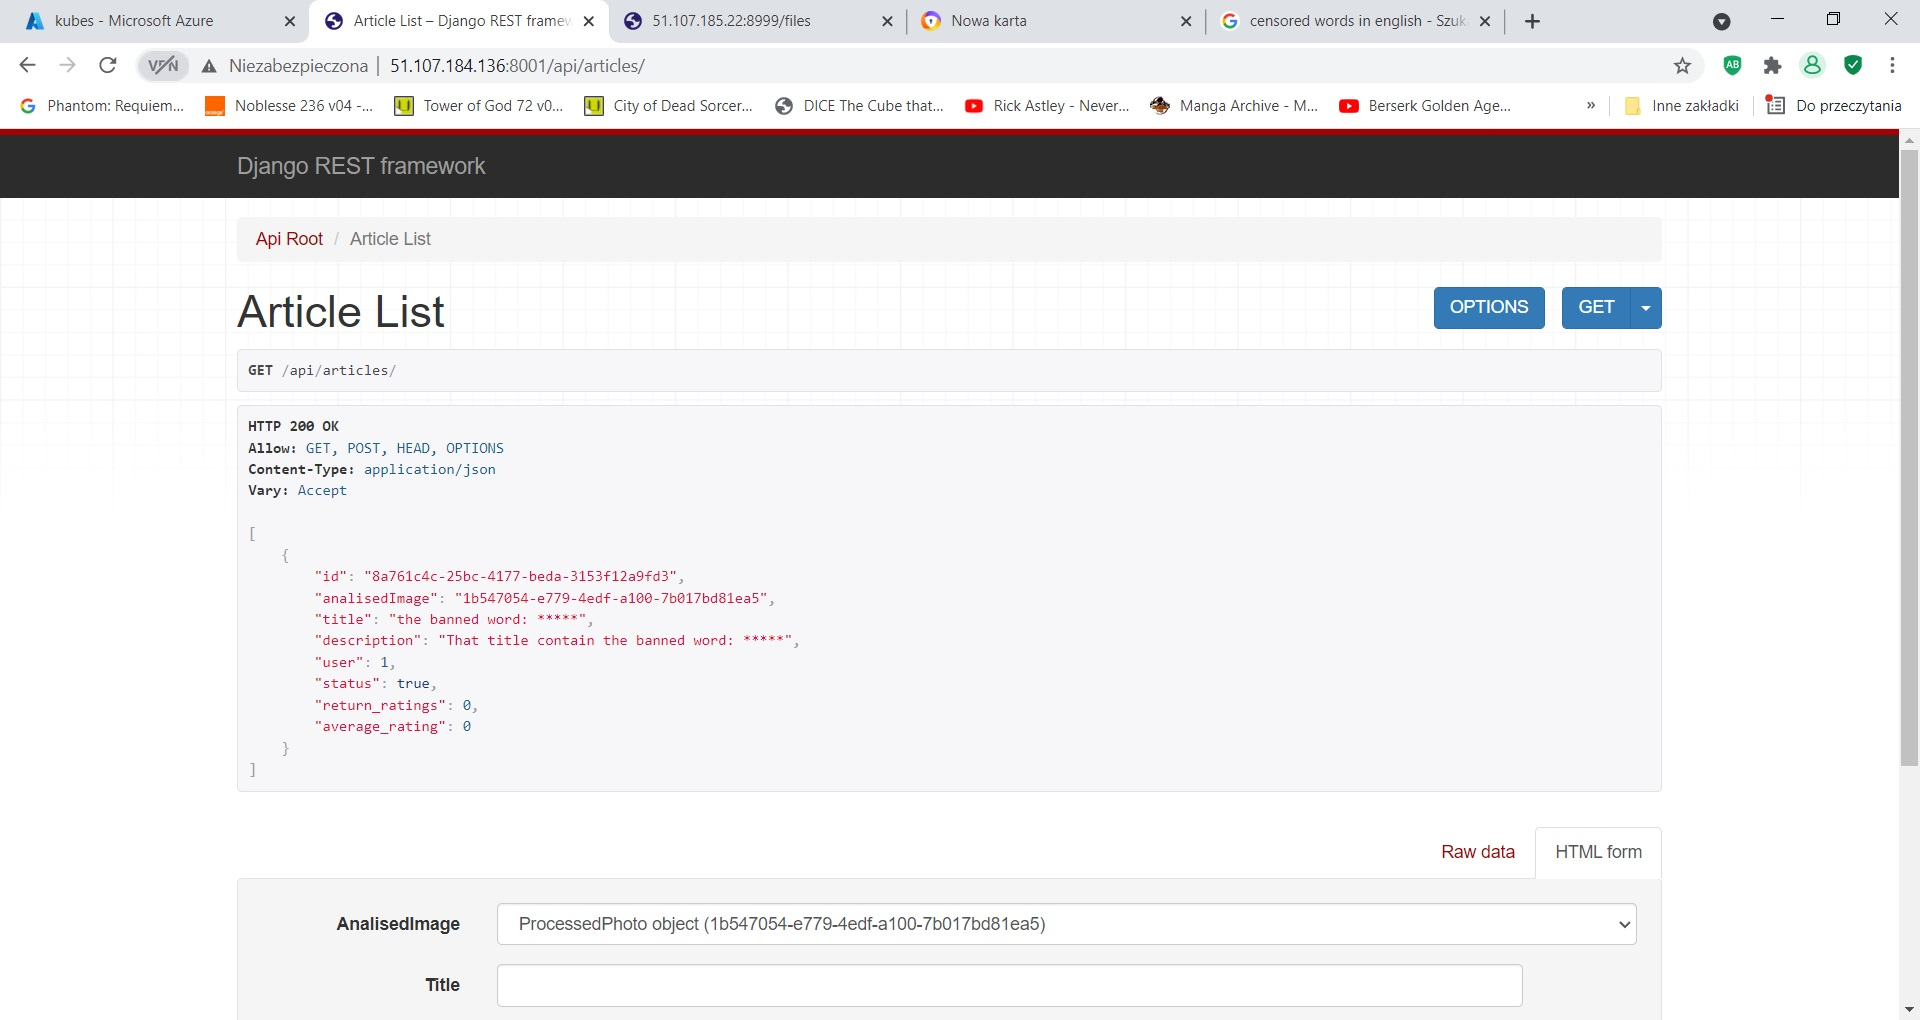
\includegraphics[width=11cm]{figures/blog3.jpg}
	\caption{Treść artykułu po cenzurze}
\label{Fig:blog3}
\end{figure}
\begin{figure}[ht]
	\centering
	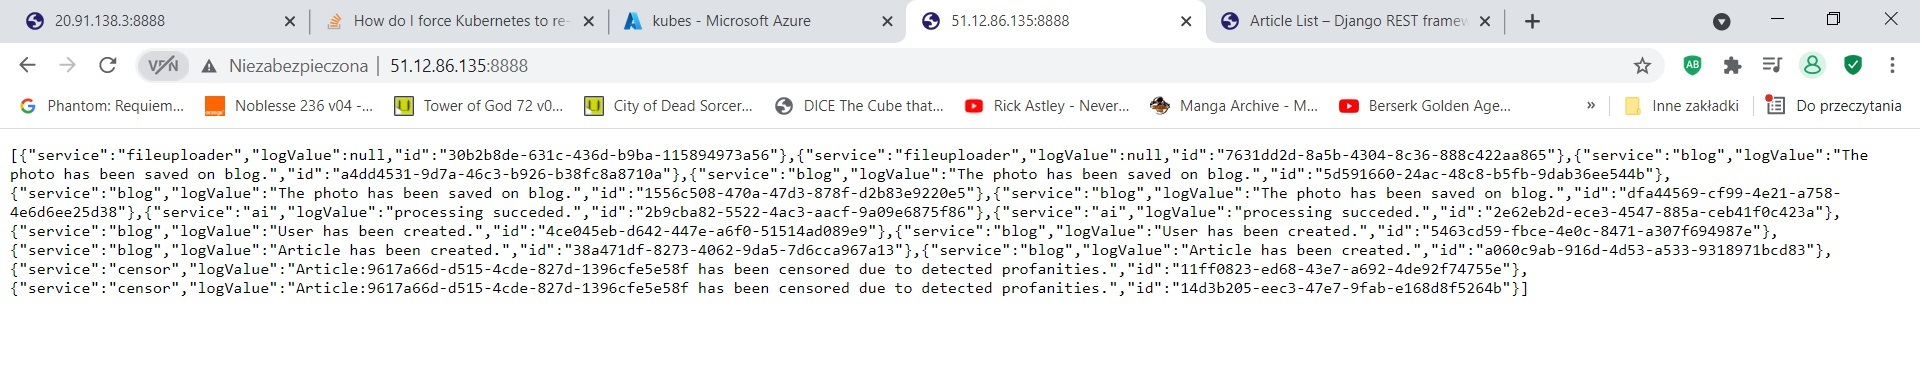
\includegraphics[width=11cm]{figures/logs.jpg}
	\caption{Efekt pracy dziennika zdarzeń}
\label{Fig:logs}
\end{figure}

Na koniec ukazano efekt pracy serwisu dziennika zdarzeń. Rysunek \ref{Fig:logs} ukazuje zdarzenia wewnątrz stosu, o których serwis został poinformowany. Informacje dotyczące wydarzeń zostały zapisane w bazie danych.
\subsection{Sposób sprawdzenia uzyskanego stosu}

Na koniec sprawdzono właściwości i możliwości stosów aplikacyjnych oraz użytych technologii. Polegały one na sprawdzeniu zachowania aplikacji przy wykorzystaniu możliwości udostępnianych przez utworzone środowiska uruchomieniowe. W ramach sprawdzenia aplikacji z użyciem konteneryzacji bez klastra przetestowano komunikację pomiędzy aplikacjami uruchomionymi oddzielnie przez \texttt{docker} oraz przy użyciu narzędzia \texttt{docker compose}. Do uruchomienia aplikacji wykorzystano komendy:
\begin{lstlisting}
docker build -t "nazwa-obrazu" --name "nazwa-kontenera" "sciezka/."
docker run -p "port:port" "nazwa-obrazu" -d
docker stop "nazwa-kontenera"
docker-compose up
docker-compose down
\end{lstlisting}
W ramach pojedyńczego uruchomienia usługi \texttt{postgres} zmieniono tymczasowo plik \texttt{dockerfile}. Usunięto z niego dodawanie pliku inicjalizacyjnego, ponieważ nie udawało się uruchomić instancji obrazu, gdy ten występował. W stosie \texttt{docker-compose} problem ten nie wystepował.

Testy oraz wdrożenie aplikacji w ramach wdrażania w \texttt{kubernetes} lokalny i globalny wykonano przez zastosowanie komend. Za znakiem  \verb|#| znajduje się opis, tego, co wykonuje dana komenda.
\begin{lstlisting}[breaklines]
kubectl apply -f "sciezka_pliku_wdrozenia" #wdraza zasob w #klaster
kubectl get pods #zbiera liste podow
kubectl get deployments # lista wdrozen
kubectl get services #zbiera liste serwisow wraz z 
#udostepnionymi portami i typem serwisu
kubectl logs "nazwa-podu" #zbiera logi aplikacji
kubectl edit deployment "nazwa-wdrozenia" #interaktywna zmiana 
#aktualnie wykorzystywanego wdrozenia -  bez zmiany pliku 
#zrodlowego wdrozenia(zmienia plik w kubernetes, nie plik, 
#ktory aplikowal)
kubectl scale deploy --replicas="liczba_podow" "nazwa-wdrozenia" #zmienia liczbe podow we wdrozeniu
kubectl describe "zasob np. deploy/pod/pods/" #szersze 
#informacje o okreslonym zasobie
kubectl delete "zasob"
kubectl config get-contexts # listuje konfiguracje dostepnych 
#klasterow dla polecenia kubectl
kubectl config use-context "nazwa kontekstu" #wybiera kontekst, 
#zmienia klaster i konfiguracje na okreslony, 
#pozwala na zmiane z klastra lokalnego na globalny i na odwrot
\end{lstlisting}

Sprawdzono jak aplikacja zachowuje się  przy instalacji zależnych wdrożeń bez ich zależności, zmniejszania i zwiększania liczby wdrożonych \texttt{podów}, sprawdzenia co się dzieje z nowym wdrożeniem, zmiany wdrożeń, usuwania określonych zasobów i wielu innych funkcjonalności które udostępniają zastosowania opisane w kolejnym rozdziale.

\subsection{Zastosowania przy tworzeniu i wdrażaniu aplikacji webowych}

Podczas pracy wykryto wiele zastosowań i przeciwwskazań do korzystania z mikroserwisów i konteneryzacji. Praca przy użyciu architektury mikroserwisowej dała wiele możliwości, które ciężko uzyskać w aplikacji monolitowej. Aplikację napisano w oparciu o podejście tworzenia obsługi tylko określonych elementów domenowych przez określony mikroserwis, co pozwoliło na skupienie się na implementacji logiki biznesowej fragmentu całego systemu. Dzięki temu uzyskano bezpośrednie dodawanie funkcjonalności biznesowych, które planowano osiągnąć. Pominięto tutaj proces zastanawiania się w jaki sposób zaimplementować rzeczy nienaturalne dla wykorzystywanego języka programowania. Użycie mikroserwisów pozwoliło na utworzenie fragmentu funkcjonalności w języku, który dany problem łatwo rozwiązał. Na podstawie tego stwierdzono, że w skonteneryzowanej architekturze mikroserwisowej nie ma problemu z połączeniem dwóch różnych stosów technologicznych. Pozbyto się problemów typu co zrobić z niewspółpracującymi technologiami, ile kodu należy zmienić, aby dodać nową funkcjonalność, zważając na ograniczenia wcześniej napisanego oprogramowania oraz czy jest to w ogóle wykonalne. 

Głównym zastosowaniem uzyskanym w pracy inżynierskiej przez użycie architektury mikroserwisowej jest podzielenie jednolitej aplikacji — bloga udostępniającego analizę przy użyciu sztucznej inteligencji dodawanych do niego obrazów oraz cenzurę artykułów do osobnych mikroserwisów pełniących określone funkcje. Dzięki temu utworzone aplikacje mają charakter ogólny — są łatwe w modyfikacji i mogą zostać ponownie użyte w przyszłości w innych systemach przez wprowadzenie małych zmian. Pozytywnym efektem ubocznym korzystania z tego podejścia jest nieustannie rosnąca biblioteka użytecznego i łatwego w zrozumieniu kodu.

Dodatkowo wprowadzono podejście pisania funkcjonalności biznesowych zamiast obsługi wszystkich określonych elementów systemu. Udało się dojść do wniosków, że w podejściu mikroserwisowym zawsze istnieje możliwość napisania dodatkowego punktu końcowego lub producenta, który przekaże odpowiednie dane. Przez to możliwe jest oddanie niepasujących domenowo funkcji biznesowej oddzielnemu modułowi, który zajmie się dokładnie tym problemem.

Zaczynając pracę wiele czasu zmarnowano na zastanawianie się nad ograniczeniami wykorzystywanych bibliotek. Po określeniu funkcjonalności niemożliwe zdawało się znalezienie sposobu na dodanie konsumenta w frameworku \texttt{django}. Konsument powinien być w pętli nieskończonej, a \texttt{django} nie pozwala na wykorzystanie ich wewnątrz siebie z powodów implementacyjnych. Po jakimś czasie jedyne rozwiązania jakie odnajdowano to dodanie brokera wiadomości \texttt{redis} i kolejki zadań \texttt{celery}, które działając wspólnie pozwalają na uruchamianie nowych procesów nieskończonych. Rozwiązanie to wnosi w system dwa dodatkowe elementy, które wymagają znajomości sposobu ich działania oraz zasobów wymaganych na wdrożenie i użycie ich. Rozwiązanie to wydawało się zbyt kosztowne pod względem zastosowania w tak małym projekcie. Wykorzystując możliwość architektury mikroserwisowej, obowiązki uruchomienia tych procesów przekazano do innych, oddzielnych mikroserwisów, przez co ograniczenia frameworku zostały ominięte.

Podział systemu na kilka mikroserwisów pozwolił również na zmniejszenie obciążenia całego systemu. W architekturze monolitycznej\footnote{architektura monolityczna — podejście zakładające tworzenie aplikacji jako jednego, zwięzłego systemu. Tradycyjne podejście do tworzenia oprogramowania.} często istnieje element, który jest nieustannie wykorzystywany przez cały system. Mikroserwisy pozwalają na odseparowanie tego elementu i uruchomienie go osobno, gdzie odseparowanym obciążeniem zajmujemy się w wielu instancjach. 

W sytuacji, gdy cały system obsługuje jeden serwer dawałoby to niewielkie przychody, a czasem nawet straty, ponieważ współdzielone zasoby są ograniczone, a każda instancja posiada własne biblioteki, które są kolejny raz wczytywane do pamięci w ramach innego mikroserwisu. Efekty działania najlepiej widać, kiedy wiele maszyn uruchamia różne procesy i współmiernie dzieli zasoby i obciążenie w klastrze \texttt{kubernetes}.

Do wprowadzenia tych możliwości wykorzystano konteneryzację i wdrożenie aplikacji w chmurę. Dzięki temu osiągnięto główne zastosowanie architektury mikroserwisowej. Przy pisaniu pracy udało się uruchomić dodatkową instancję pojedynczego mikroserwisu który był bardzo obciążony. Zamiast uruchamiania całości aplikacji blogu po raz kolejny na nowym serwerze uruchomiono pojedynczą usługę, która wymaga dodatkowego wsparcia. Jest to olbrzymia zaleta, ponieważ zamiast mnożyć zasoby używane przez system, można dodawać je w osobnych \texttt{podach}. Dodatkowo, wykorzystanie z usług chmurowych powoduje, że płacimy za używane zasoby, a nie maszyny fizyczne. Użycie tego stosu technologicznego w rozwiązaniu chmurowym pozwoliło na całkowite uniezależnienie systemu od implementacji fizycznej zasobów. Nie było konieczności zastanawiania się, czy możemy dostawić kolejny serwer, jakie parametry należy wybrać, gdzie powinien się mieścić, jaki serwer wybrać.
 
Niestety podczas pisania aplikacji nie udało się pozbyć zależności pomiędzy mikroserwisami. Udało się odseparować te zależności tylko do fragmentów mikroserwisów wymagających współpracy do funkcjonowania. Uruchomienie usług bloga, dziennik zdarzeń oraz przesyłu plików nie jest zależne od tego, czy inny mikroserwis funkcjonuje w chwili ich działania. Uruchomienie innego mikroserwisu nie jest potrzebne, aby one działały. Pośredniczący serwis sztucznej inteligencji przetwarza pliki tylko wtedy, gdy oba mikroserwisy funkcjonują. Udało się odseparować funkcjonalności w taki sposób, aby łatwo było określić czym zajmuje się każdy mikroserwis. Blog jest prostym blogiem, a nie wszechstronną aplikacją przetwarzającą zdjęcia przy użyciu sztucznej inteligencji i sprawdzającą, czy treści są niecenzuralne. Efektem ubocznym tej implementacji są mikroserwisy, które nie mogą funkcjonować w przypadku awarii lub błędu innego mikroserwisu. Udało się jednak zmniejszyć wagę tego problemu wprowadzając orkiestrację przy użyciu \texttt{kubernetes}, który automatycznie uruchamiał \texttt{pody} w przypadku ich awarii. W efekcie serwisy podległe zostały uruchomione, gdy tylko awaria usługi, od której były zależne została naprawiona.

Kolejnym problemem wykrytym w pracy jest brak wspólnej pamięci. Przy testowaniu bazy danych w środowisku lokalnym z wieloma wolumenami zauważono, że bazy danych posiadają różny stan. Zależnie od tego która instancja bazy danych została uzyskiwane były różne zawartości. Działo się to nawet, gdy wykorzystano wolumen wspólny. Ukazało to, że aplikacje posiadające stan zachowany w pamięci nie nadają się do bezpośredniego wprowadzenia w \texttt{kubernetes}. Rozwiązaniem tego problemu może być wprowadzenie operatorów, które będą nadzorować stan obsługiwanej usługi stanowej. Istnieją gotowe rozwiązania bazy danych\cite{PostgresOperator, ZalandoOperator} jednak wymagają one dokładnej znajomości tematu, wprowadzenia szyfrowania haseł przy użyciu sekretów, wprowadzenia konfiguracji połączeń szyfrowanych do każdego mikroserwisu oraz wielu innych konfiguracji, których zakres był zbyt szeroki aby opisać go w ramach tej pracy dyplomowej.

Głównym zastosowaniem konteneryzacji było uzyskanie przenośności kodu, separacja środowiska i centralizacja konfiguracji. Dodatkowo, dzięki konteneryzacji udało się pobrać i zainstalować narzędzia z domyślną konfiguracją za pomocą jednej linijki kodu. Co więcej, skorzystanie z konteneryzacji zapewniło bezpieczeństwo środowiska lokalnego przy rozwoju aplikacji od efektów ubocznych pozostałych aplikacji, które były skonteneryzowane.

Po długotrwałych testach i poszukiwaniach nie udało się wprowadzić funkcjonalnego sposobu na udostępnienie dostępu do środowiska lokalnego kontenerowi, głównie z powodu braku doświadczenia i odpowiedniej wiedzy koniecznej do wykonania tego. Jednak nie była to strata czasu, dzięki temu ustalono, że aby doznać efektów ubocznych działania \texttt{dockera} w środowisku lokalnym konieczne jest świadome działanie i dążenie do udostępnienia tej funkcjonalności.

Niestety, odpowiednie doświadczenie i współpraca z osobami, które potrafią projektować mikroserwisy jest kluczowe w tworzeniu produktu pozwalającego wykorzystać wszystkie te zastosowania. Na podstawie osobistych odczuć stwierdzono, że architektura mikroserwisowa pomimo swoich zalet jest zbyt trudnym zagadnieniem dla osoby niedoświadczonej. Konieczność znajomości wielu nowych pojęć, zagadnień, wzorców projektowych oraz zmiana podejścia do sposobu pisania oprogramowania są niesamowicie przytłaczającym doświadczeniem. Zagadnienie wymaga odpowiedniego przygotowania, umiejętnego procesu projektowania stosu mikroserwisów oraz nieustannej pracy nad zmianą wcześniej wyuczonych nawyków programowania, które utrudniają pracę w architekturze mikroserwisowej. Wymagana jest do tego osoba doświadczona i obeznana w mikroserwisach.

Zauważono, że ze względu na równoczesne przetwarzanie przez wiele \texttt{podów} utracono została domyślna właściwość architektury monolitycznej - możliwość zachowywania kolejności obsługi żądań. Implementacja mikroserwisów użyta w pracy nie zapewnia, że wcześniej rozpoczęte przetwarzanie żądania przez pewien \texttt{pod} wykona się przed zakończeniem obsługi później rozpoczętego żądania obsługiwanego w tym samym czasie. Stwierdzono, że w przypadku obsługi wielu żądań dotyczących zmiany tego samego obiektu lub dotyczącego tych samych danych należy zaimplementować dodatkowe mechanizmy zapewniające ich spójność i kolejność.

Jedynym negatywnym efektem konteneryzacji, który zauważono jest trudność w tworzeniu własnych schematów obrazów i konfiguracji kontenerów dla osób z małym doświadczeniem programistycznym. Znajomość tego w jaki sposób dana komenda wpływa na obraz była kluczowa w utworzeniu aplikacji, która będzie działać prawidłowo w tym środowisku. Niestety, ze względu na małe doświadczenie nie uniknięto utraty cennych godzin na walkę z problemami związanymi z nieprawidłowym zrozumieniem lub wykorzystaniem komend. Główny problem sprawiało dostosowanie adresów sieciowych oraz punktu wyjścia pozwalającego na przeprowadzenie migracji bazy danych po zapewnieniu jej inicjalizacji. Na podstawie tego stwierdzono, że pewne zdolności programistyczne i głębsza znajomość sposobu działania sieci są kluczowe w operowaniu konteneryzacją.

Zdolność do separacji środowiska programistycznego, generalizacji konfiguracji w postaci zmiennych środowiskowych oraz uproszczenie wprowadzania konfiguracji sieciowej w ramach systemów rozproszonych to rzeczy, które mogą się przydać przy tworzeniu prawie każdej aplikacji. Na podstawie doświadczeń pracy z \texttt{dockerem} i innymi rozwiązaniami konteneryzacyjnymi stwierdzono, że każda aplikacja webowa może wykorzystać konteneryzację w mniejszym lub większym stopniu w zastosowaniach wcześniej wymienionych.

Warto wspomnieć, że skonteneryzowane mikroserwisy wdrażane przy użyciu orkiestracji w klastrze \texttt{kubernetes} pozwoliły na aktualizację wersji oprogramowania bez przerwy w pracy aktualizowanej usługi. Wprowadzenie nowego wdrożenia dla tej samej definicji zasobu z inną wersją obrazu obsługującego \texttt{pod} wykonywane było jednocześnie. W trakcie wdrażania nowego obrazu poprzednie \texttt{pody} wykorzystujące starszą wersję były utrzymywane przy życiu do momentu informacji o prawidłowym funkcjonowaniu nowo wdrożonych \texttt{podów}. Jeżeli z jakiegoś powodu wdrożenie nie uda się, poprzednia wersja aplikacji ciągle działa do momentu wprowadzenia prawidłowo funkcjonalnego wdrożenia. Po wprowadzeniu wdrożenia, \texttt{Kubernetes} przekierowuje obciążenie ze starych \texttt{podów} do nowych, a na koniec zabija i usuwa stare \texttt{pody}. Taki sposób działania orkiestratora pozwolił na uniknięcie sytuacji, w której usługi stają się niedostępne z powodu wprowadzania aktualizacji systemu. Warto podkreślić, że ze względu na dostęp do fragmentów systemu - mikroserwisów nie było konieczności aktualizacji całego systemu, tak jak ma to miejsce w monolitowym podejściu. Udało się wykonać zarówno pojedyncze wdrożenie nowej wersji pojedynczego mikroserwisu, jak i wdrożenie równoległe wielu mikroserwisów jednocześnie. 

Poprzednio wspomniany mechanizm zapewnił, że nadmiarowość systemu w trakcie aktualizacji usługi jest skrócona do minimalnego, potrzebnego na to okresu. Do udostępnienia tych same możliwości w monolitycznym podejściu, konieczne byłoby uruchomienie kolejnej instancji całego systemu, co bardzo często okazuje się mniej opłacalne niż wyłączenie go na czas aktualizacji.
\clearpage

\section{Podsumowanie i wnioski końcowe}

W ramach pracy udało się utworzyć i uruchomić w lokalnym środowisku stos mikroserwisów. Następnie wykorzystano \texttt{docker} \texttt{docker-compose} w celu jego konteneryzacji. Przy użyciu \texttt{kubernetes}  udało się wdrożyć stos skonteneryzowanych mikroserwisów w klaster publiczny zgodnie z założeniami. Następnie wykorzystano dany stos do sprawdzenia zastosowań mikroserwisów i konteneryzacji w tworzeniu i wdrażaniu aplikacji webowej.

Na podstawie osiągniętych wyników wyciągnięto wniosek, że architektura mikroserwisowa ma zastosowanie przy tworzeniu rozproszonej aplikacji webowej o wysokiej skalowalności i podzielonej na małe, łatwo utrzymywalne, rozwijalne i rozdzielnie wdrażane elementy, jednak wymagane są do tego osoby doświadczone. Na podstawie uzyskanych doświadczeń przy tworzeniu pracy stwierdzono, że projektowanie i konfiguracja tworzonego stosu była procesem długotrwałym i trudnym, tworzącym wiele błędów i wymagającym dokładnego zrozumienia tego, co chce się osiągnąć wprowadzając ją, dlatego niezalecane jest wykorzystanie jej, jeśli produkt chcemy wydać jak najszybciej. Wprowadzenie mikroserwisów uprościło pisanie kodu dopiero po nabraniu doświadczenia zarówno zawodowego, jak i przy pisaniu pracy. Dlatego zdaniem autora tej pracy nie zaleca się tworzenia nowej aplikacji jako produkt bez odpowiedniego przygotowania i napisania kilku aplikacji w tej architekturze. Osoba niedoświadczona może nie być świadoma przy jak dużej aplikacji wprowadzenie mikroserwisów będzie opłacalne. Bardzo często może się okazać, że wprowadzenie uproszczenia pisania elementów aplikacji tak naprawdę wydłuża czas produkcji przez odpowiednie projektowanie sposobu połączeń i zależności mikroserwisów.

Wykorzystując konteneryzację określono, że jest to narzędzie, które może być wykorzystywane przy każdym tworzeniu i wdrożeniu aplikacji webowej. Serwer może uruchomić kontener, którego porty zostaną zmapowane na porty serwera. Dodatkowo wykorzystanie konteneryzacji umożliwiło wprowadzenie aplikacji w usługi klastera \texttt{kubernetes}, który automatycznie skalował aplikację przez uruchamianie i wyłączanie instancji węzłów obsługujących instancje wdrożonej aplikacji.

Autor za własny wkład pracy uważa:
\begin{enumerate}[label=\arabic*), leftmargin=1.25cm]
\item zebranie wiedzy koniecznej do prawidłowego zrozumienia i podejścia do tematu,
\item zaprojektowanie stosu mikroserwisów i sposobu komunikacji pomiędzy nimi,
\item konteneryzację mikroserwisów,
\item stworzenie konfiguracji klastra \texttt{kubernetes},
\item wybór środowiska wdrożeniowego,
\item wdrożenie aplikacji w chmurowy klaster \texttt{kubernetes} \texttt{Azure Kubernetes Service},
\item sprawdzenie zastosowań mikroserwisów oraz konteneryzacji w tworzeniu i wdrożeniu wykonanej aplikacji.
\end{enumerate}

\clearpage
\section*{Załączniki}
\addcontentsline{toc}{section}{Załączniki}

Razem z pracą inżynierską został załączony folder zawierający kod źródłowy stosu zaimplementowanych mikroserwisów wraz z plikami \texttt{dockerfile} i \texttt{docker-compose} pozwalającymi na utworzenie obrazów i stosu \texttt{dockerowego}, oraz pliki wdrożeniowe.
\clearpage

\addcontentsline{toc}{section}{Literatura}

\begin{thebibliography}{4}
\bibitem{fowler}https://martinfowler.com/microservices/, Dostęp 01.01.2022.
\bibitem{fowler2}https://martinfowler.com/articles/microservices/, Dostęp 01.01.2022.
\bibitem{virtualisation}https://pl.euro-linux.com/blog/slowniczek-pojec-wirtualizacja-konteneryzacja-cloud, Dostęp 01.01.2022.
\bibitem{differences}https://www.baeldung.com/cs/virtualization-vs-containerization, Dostęp 01.01.2021.
\bibitem{cluster}https://www.redhat.com/en/topics/containers/what-is-a-kubernetes-cluster, Dostęp 01.01.2022.
\bibitem{thoughtwork}https://www.thoughtworks.com/what-we-do, Dostęp 01.01.2022.
\bibitem{thdocker}https://www.thoughtworks.com/radar/platforms/docker, Dostęp 01.01.2022.
\bibitem{thkubernetes}https://www.thoughtworks.com/radar/platforms/kubernetes, Dostęp 01.01.2022.
\bibitem{thservices}https://www.thoughtworks.com/radar/techniques/microservices, Dostęp 01.01.2022.
\bibitem{thenvy}https://www.thoughtworks.com/radar/techniques/microservice-envy, Dostęp 01.01.2022.
\bibitem{thlayered}https://www.thoughtworks.com/radar/techniques/layered-microservices-architecture, Dostęp 01.01.2022.
\bibitem{uses}https://microservices.io/articles/whoisusingmicroservices.html, Dostęp 01.01.2022.
\bibitem{future}https://wiredelta.com/10-reasons-why-microservices-are-the-future/, Dostęp 01.01.2022.
\bibitem{future2}https://www.hospitalitynet.org/opinion/4107609.html, Dostęp 01.01.2022.
\bibitem{future3}https://softclouds.medium.com/the-future-of-software-development-with-microservices-5f4d263272b0, Dostęp 01.01.2022.
\bibitem{future4}https://devops.com/how-ai-and-microservices-create-a-reliable-enterprise-of-the-future/, Dostęp 01.01.2022.
\bibitem{Richardson} Richardson C.: Microservices Patterns, Manning Publications, 2018.
\bibitem{stranglerFowler}https://martinfowler.com/bliki/StranglerFigApplication.html, Dostęp 01.01.2022.
\bibitem{strangler}http://paulhammant.com/2013/07/14/legacy-application-strangulation-case-studies/, Dostęp 01.01.2022.
\bibitem{sub}https://www.docker.com/blog/updating-product-subscriptions/, Dostęp 01.01.2022.
\bibitem{kubernetesInAction}Lukša M.: Kubernetes in Action, Manning Publications, 2018.
\bibitem{eventDrivenMicroservices} Bellemare A.: Building Event-Driven Microservices: Leveraging Organizational Data at Scale, O'Reilly, 2020.
\bibitem{registry}https://blog.sonatype.com/how-to-get-started-with-nexus-repository-manager-oss, Dostęp 01.01.2022.
\bibitem{kubernetes}https://kubernetes.io/pl/docs/concepts/overview/what-is-kubernetes/, 01.01.2022.
\bibitem{services}https://kubernetes.io/docs/concepts/services-networking/service/, Dostęp 01.01.2022.
\bibitem{lib}https://github.com/smahesh29/Gender-and-Age-Detection, Dostęp 01.01.2022.
\bibitem{pf}https://pypi.org/project/profanity-filter/, Dostęp 01.01.2022.
\bibitem{kafka}https://kafka.apache.org/, Dostęp 01.01.2022.
\bibitem{confluent}https://github.com/confluentinc/confluent-kafka-python, Dostęp 01.01.2022.
\bibitem{kafka-python}https://kafka-python.readthedocs.io/en/master/, Dostęp 01.01.2022.
\bibitem{myhub}https://hub.docker.com/search?q=bfinger1997, Dostęp 01.01.2022.
\bibitem{bitnami}https://github.com/bitnami/bitnami-docker-kafka/blob/master/docker-compose.yml, Dostęp 01.01.2022.
\bibitem{kafkadcc}https://raw.githubusercontent.com/bitnami/bitnami-docker-kafka/master/docker-compose.yml, Dostęp 01.01.2022.
\bibitem{hub}https://hub.docker.com/, Dostęp 01.01.2022.
\bibitem{helm}https://bitnami.com/stack/kafka/helm, Dostęp 01.01.2022.
\bibitem{PostgresOperator}https://access.crunchydata.com/documentation/postgres-operator/latest/, Dostęp 09.01.2022.
\bibitem{ZalandoOperator}https://github.com/zalando/postgres-operator, Dostęp 09.01.2022.


\end{thebibliography}

\clearpage

\makesummary

\end{document} 